\documentclass{tietreport}

% Import images
\usepackage{graphicx}

% Rotate wide diagrams onto landscape pages
\usepackage{pdflscape}

% Keep each figure directly under its section heading
\usepackage{float}

% Bibliography: not used yet (no references cited in the mid-semester report).
% Uncomment this block, add references.bib and \printbibliography at the end
% when you start citing sources for the final evaluation.
%\usepackage[
%  date=year,
%  style=alphabetic,
%  backend=biber,
%  sorting=nty,
%  maxnames=5,
%  minnames=3,
%  maxalphanames=4,
%  minalphanames=3,
%  backref=true,
%  doi=false,
%  isbn=false,
%  url=false,
%  eprint=false
%]{biblatex}
%\addbibresource{references.bib}

%% ==================================================
%% CUSTOMIZE THESE FIELDS FOR YOUR PROJECT
%% ==================================================

% Course/Lab header
\TitlePageHeader{%
  UCS503 - Software Engineering%
}

% Main project title
\ProjectTitle{%
  MediSynth%
}

% Subtitle or project description
\ProjectSubTitle{%
  A Hospital Management System with a
  Privacy-Preserving Synthetic Patient Data
  Engine (SynthetiX)%
}

% Student information (up to 4 students)
\author{%
  \texttt{1024030787} Aryan Sharma \\
  \texttt{1024030792} Brahmdeep Singh Khanuja \\
  \texttt{1024030793} Keerat Singh Brar%
}

% Group number, degree, year, program
\TitlePageSubText{%
  Group: \texttt{3C55} BE Third Year, COE%
}

% Faculty advisor/guide name
\AdvisorName{%
  Ms. Nisha Thakur%
}

% Evaluation period and department info
\TitlePageFooterText{{%
    \large Mid-Semester Evaluation \\[0.2cm]
    \bfseries Computer Science and Engineering
    Department%
  } \\[0.15cm]
  Thapar Institute of Engineering and Technology,
  Patiala%
}

%% ==================================================

\begin{document}

% Generate title page
\maketitle

% Table of contents (auto-generated from chapters)
\tableofcontents

% ===== CHAPTER 1: INTRODUCTION =====

\chapter{Introduction}

\section{Background and Context}

Hospital software teams increasingly need realistic
patient data to build, test, and demonstrate new
systems before they can be deployed. This need
extends beyond production hospitals to academic and
research settings, where teams frequently have no
legitimate way to access real patient records at
all. Real patient data is protected health
information under regulations such as HIPAA (United
States) and India's Digital Personal Data Protection
(DPDP) Act, and cannot legally or ethically be
shared with developers, students, or third-party
testers without extensive data-use agreements that
are impractical within a single academic semester.

MediSynth addresses this gap by pairing a fully
functional hospital management system (HMS) with
Synthetix, a synthetic patient data engine. Rather
than relying on real records or simple field-masking,
Synthetix generates entirely new, artificial patient
data that preserves the statistical patterns found
in real healthcare data---age-diagnosis correlations,
prescription frequencies, appointment
volumes---without representing any real individual.
This lets our team, and potentially others in a
similar position, build and validate a realistic
hospital system without ever touching protected data.

\subsection{Problem Statement}

Student and early-stage development teams building
healthcare software face four related obstacles:

\begin{itemize}
  \item \textbf{Legal restriction:} real hospital
    records fall under HIPAA and the DPDP Act;
    hospitals cannot hand them to student developers
    or third-party testers without extensive data-use
    agreements that are impractical within a single
    semester.
  \item \textbf{Re-identification risk:} simple
    anonymization (removing names or ID numbers) is
    frequently reversible---prior research has shown
    that a large majority of a population can be
    uniquely re-identified from just three seemingly
    harmless fields such as date of birth, gender,
    and postal code. This makes basic field-masking
    an unreliable substitute for genuine privacy
    protection.
  \item \textbf{Unrealistic test data:} teams that
    avoid real data often fall back on small,
    hand-typed mock records that do not reflect real
    clinical patterns, producing systems that are
    never properly stress-tested before deployment.
  \item \textbf{Fragmented development:} without a
    single, realistic, shared dataset, each part of a
    hospital system---backend, frontend, mobile,
    analytics---tends to invent its own inconsistent
    mock data, causing integration rework later in
    the project.
\end{itemize}

MediSynth's core engineering problem is therefore
twofold: build a complete, role-based hospital
management system, and build a data engine capable of
seeding that system with statistically realistic,
privacy-safe data from day one of development.

\section{Project Objectives}

\begin{enumerate}
  \item Deliver a functional, role-based Hospital
    Management System covering patient registration,
    appointment booking, doctor consultation, medical
    records, prescriptions, lab test workflows, and
    billing, built and integrated across four
    coordinated lanes (backend, frontend, mobile,
    data engine) within the 10-week project timeline.
  \item Design and implement Synthetix, a statistical
    synthetic-data generation engine that produces a
    patient dataset (target size: 10,000 records) with
    zero real patient records, validated by comparing
    key summary statistics of the generated data
    against reference public healthcare distributions
    before each release.
  \item Establish a working CI/CD pipeline that
    automatically builds and tests all four lanes on
    every change and deploys to a staging environment,
    so that a working, seeded, role-based demo of the
    system is available by the mid-semester
    evaluation.
\end{enumerate}

These objectives were chosen to be measurable at this
stage of the project: Objective 1 and 3 are directly
demonstrable in the current submission, while full
validation of Objective 2's statistical fidelity
target will be reported in the final evaluation once
the complete synthetic dataset has been generated and
benchmarked.

% ===== CHAPTER 2: METHODOLOGY & DESIGN =====

\chapter{Methodology and Design}

\section{System Architecture}

\subsection{High-Level Design}

MediSynth is built across four coordinated lanes that
share a common PostgreSQL schema:

\begin{itemize}
  \item \textbf{Backend (Java with Spring Boot):}
    exposes REST APIs for authentication, patient and
    appointment management, medical records,
    prescriptions, and billing. Implements JSON Web
    Token (JWT) based authentication and role-based
    access control (RBAC) so that admin, doctor, lab
    technician, pharmacist, and patient roles each see
    only the actions relevant to them. All sensitive
    actions (record updates, prescription changes,
    dataset access) are written to an audit log.
  \item \textbf{Frontend (React):} the primary web
    interface used by hospital staff---admin
    dashboards, doctor consultation views, and
    pharmacy/lab workflows.
  \item \textbf{Data engine (Synthetix, Python):}
    decoupled from the backend so it can be run
    independently to (re)generate a synthetic dataset
    at any time. It is the only component that ever
    writes patient-like data into the system during
    development, since no real patient data is
    available to the team.
\end{itemize}

The database uses a 13-table relational schema with
multi-tenant isolation, so that in principle multiple
hospitals could use a single deployment without any
cross-visibility of each other's data---a design
choice made early to keep the schema realistic even
though the current deployment target is a single
institution.

\subsection{Technical Stack}

\begin{itemize}
  \item \textbf{Framework/Language:} Java with Spring
    Boot (backend API); React (web frontend); Python
    (Synthetix data engine).
  \item \textbf{Database:} PostgreSQL, accessed via a
    parameterised query layer to prevent SQL
    injection.
  \item \textbf{Tools:} Git/GitHub for version
    control; GitHub Actions for CI/CD; Postman for API
    testing; draw.io for UML and data-flow design
    documentation.
  \item \textbf{Libraries:} React.js, Axios, and
    JavaScript for the frontend; Java and Spring Boot
    for the backend, with Spring Security, JWT, and
    BCrypt for authentication; and Python with pandas,
    NumPy, and SciPy for synthetic data generation.
\end{itemize}

\section{Implementation Details}

\subsection{Module 1: Core Functionality}

This module covers the functionality completed and
demonstrable at the time of this submission.

\textbf{Authentication and access control.} All API
routes are protected by JWT-based authentication
issued at login. A role-based middleware layer checks
each request against the caller's role (admin, doctor,
lab technician, pharmacist, or patient) before
allowing access, and passwords are stored using bcrypt
hashing rather than in plain text.

\textbf{Core relational schema.} The 13-table
PostgreSQL schema currently covers patients, staff
(with role), appointments, medical records,
prescriptions, and billing, with foreign-key
relationships enforcing that, for example, a medical
record cannot exist without an associated patient, and
a prescription cannot exist without an associated
medical record.

\textbf{Patient and appointment workflows.} CRUD APIs
are implemented for patient registration and login,
doctor search and selection, and appointment booking
with conflict checking against existing bookings. A
corresponding set of screens exists in the React
frontend for staff-side booking management.

\textbf{Doctor consultation and medical records.}
Doctors can view a patient's medical history and
update it with consultation notes through a dedicated
API and UI flow, forming the foundation that the
lab-test and prescription workflows (planned for
Module 2) will build on.

\textbf{Synthetix v1: rule-based synthetic data
generation.} The first version of the Synthetix
pipeline is implemented in Python as a CSV-to-CSV
generator. It profiles publicly available healthcare
statistics (age-band distributions, disease prevalence
by age group) to define sampling distributions, then
generates synthetic patient records from those
distributions rather than from any real record. This
first-pass dataset is used to seed the PostgreSQL
database so that every lane of the project has a
consistent, realistic dataset to build and test
against, instead of each lane inventing its own
inconsistent mock data.

\textbf{Audit logging.} Sensitive actions---record
creation, updates to medical records or
prescriptions---are written to an audit log table,
laying the groundwork for the fuller data-governance
features planned for later modules.

Together, these pieces form a working, seeded,
role-based slice of the system: a user can register,
log in under the correct role, book or manage an
appointment, and view or update a medical record, all
against data that Synthetix generated rather than any
real patient's information.

% ===== CHAPTER 3: DIAGRAMS =====

\chapter{Diagrams}

This chapter collects the UML and data-flow diagrams
that describe the MediSynth system: use cases, class
structure, workflows (activity and swimlane diagrams),
data flow, object interactions (sequence and
collaboration diagrams), object life cycles (state
diagrams), and the software components.

% ----- Use case -----
\section{Use Case Diagram}

\begin{figure}[H]
  \centering
  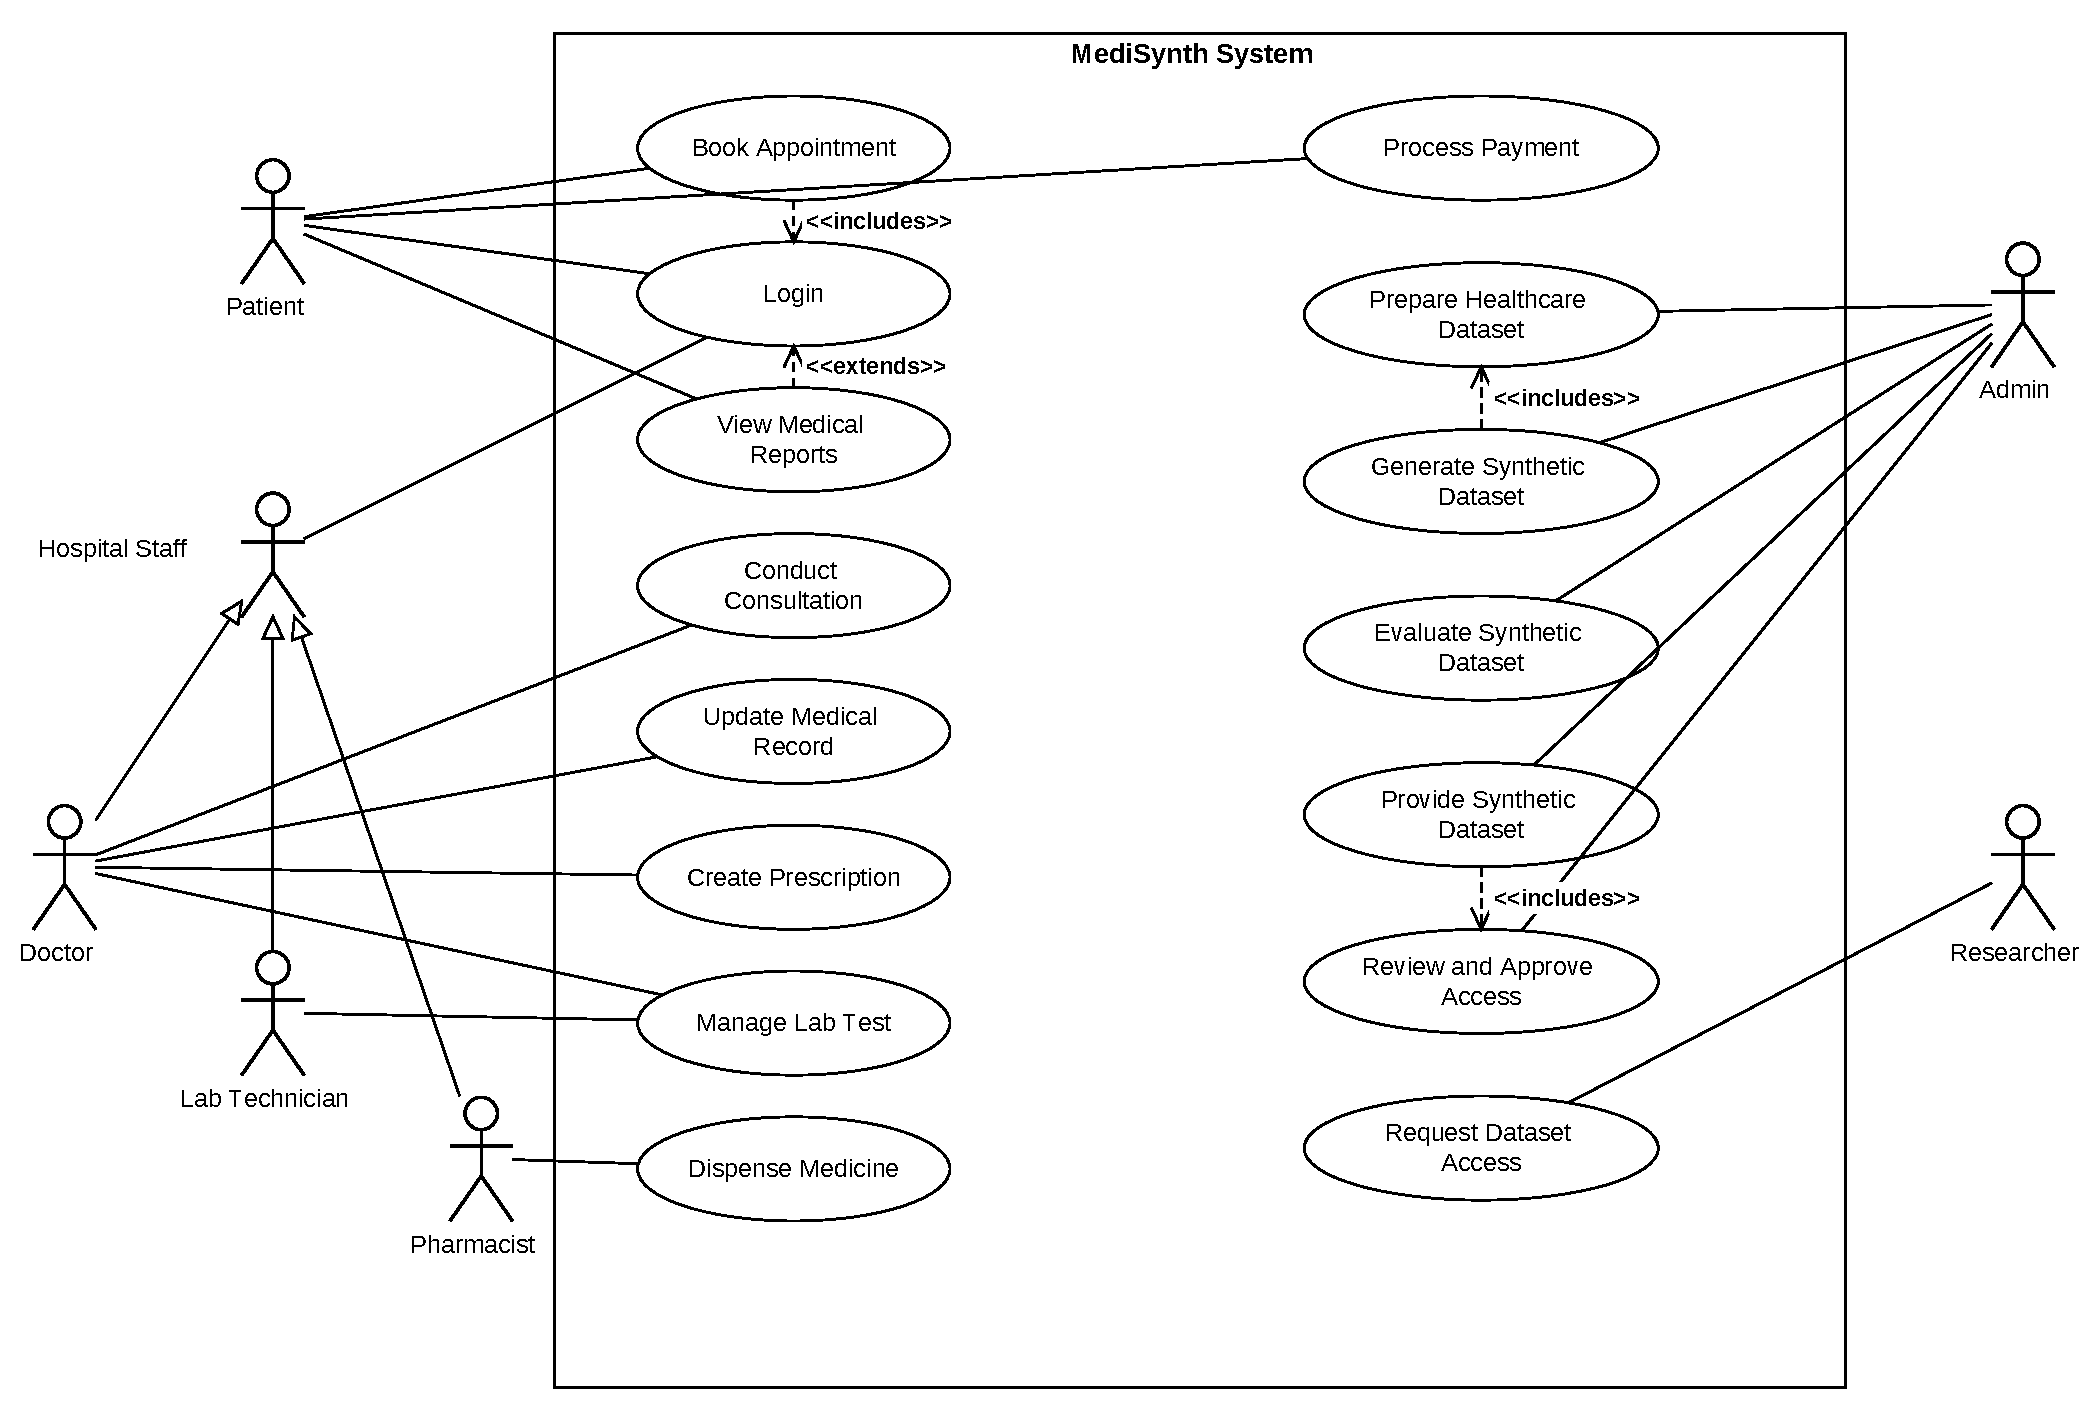
\includegraphics[width=\textwidth,height=0.72\textheight,keepaspectratio]{figures/usecase.pdf}
  \caption{Use case diagram for MediSynth}
  \label{fig:usecase}
\end{figure}
\clearpage

% ----- Class diagram -----
\begin{landscape}
\section{Class Diagram}
\begin{figure}[H]
  \centering
  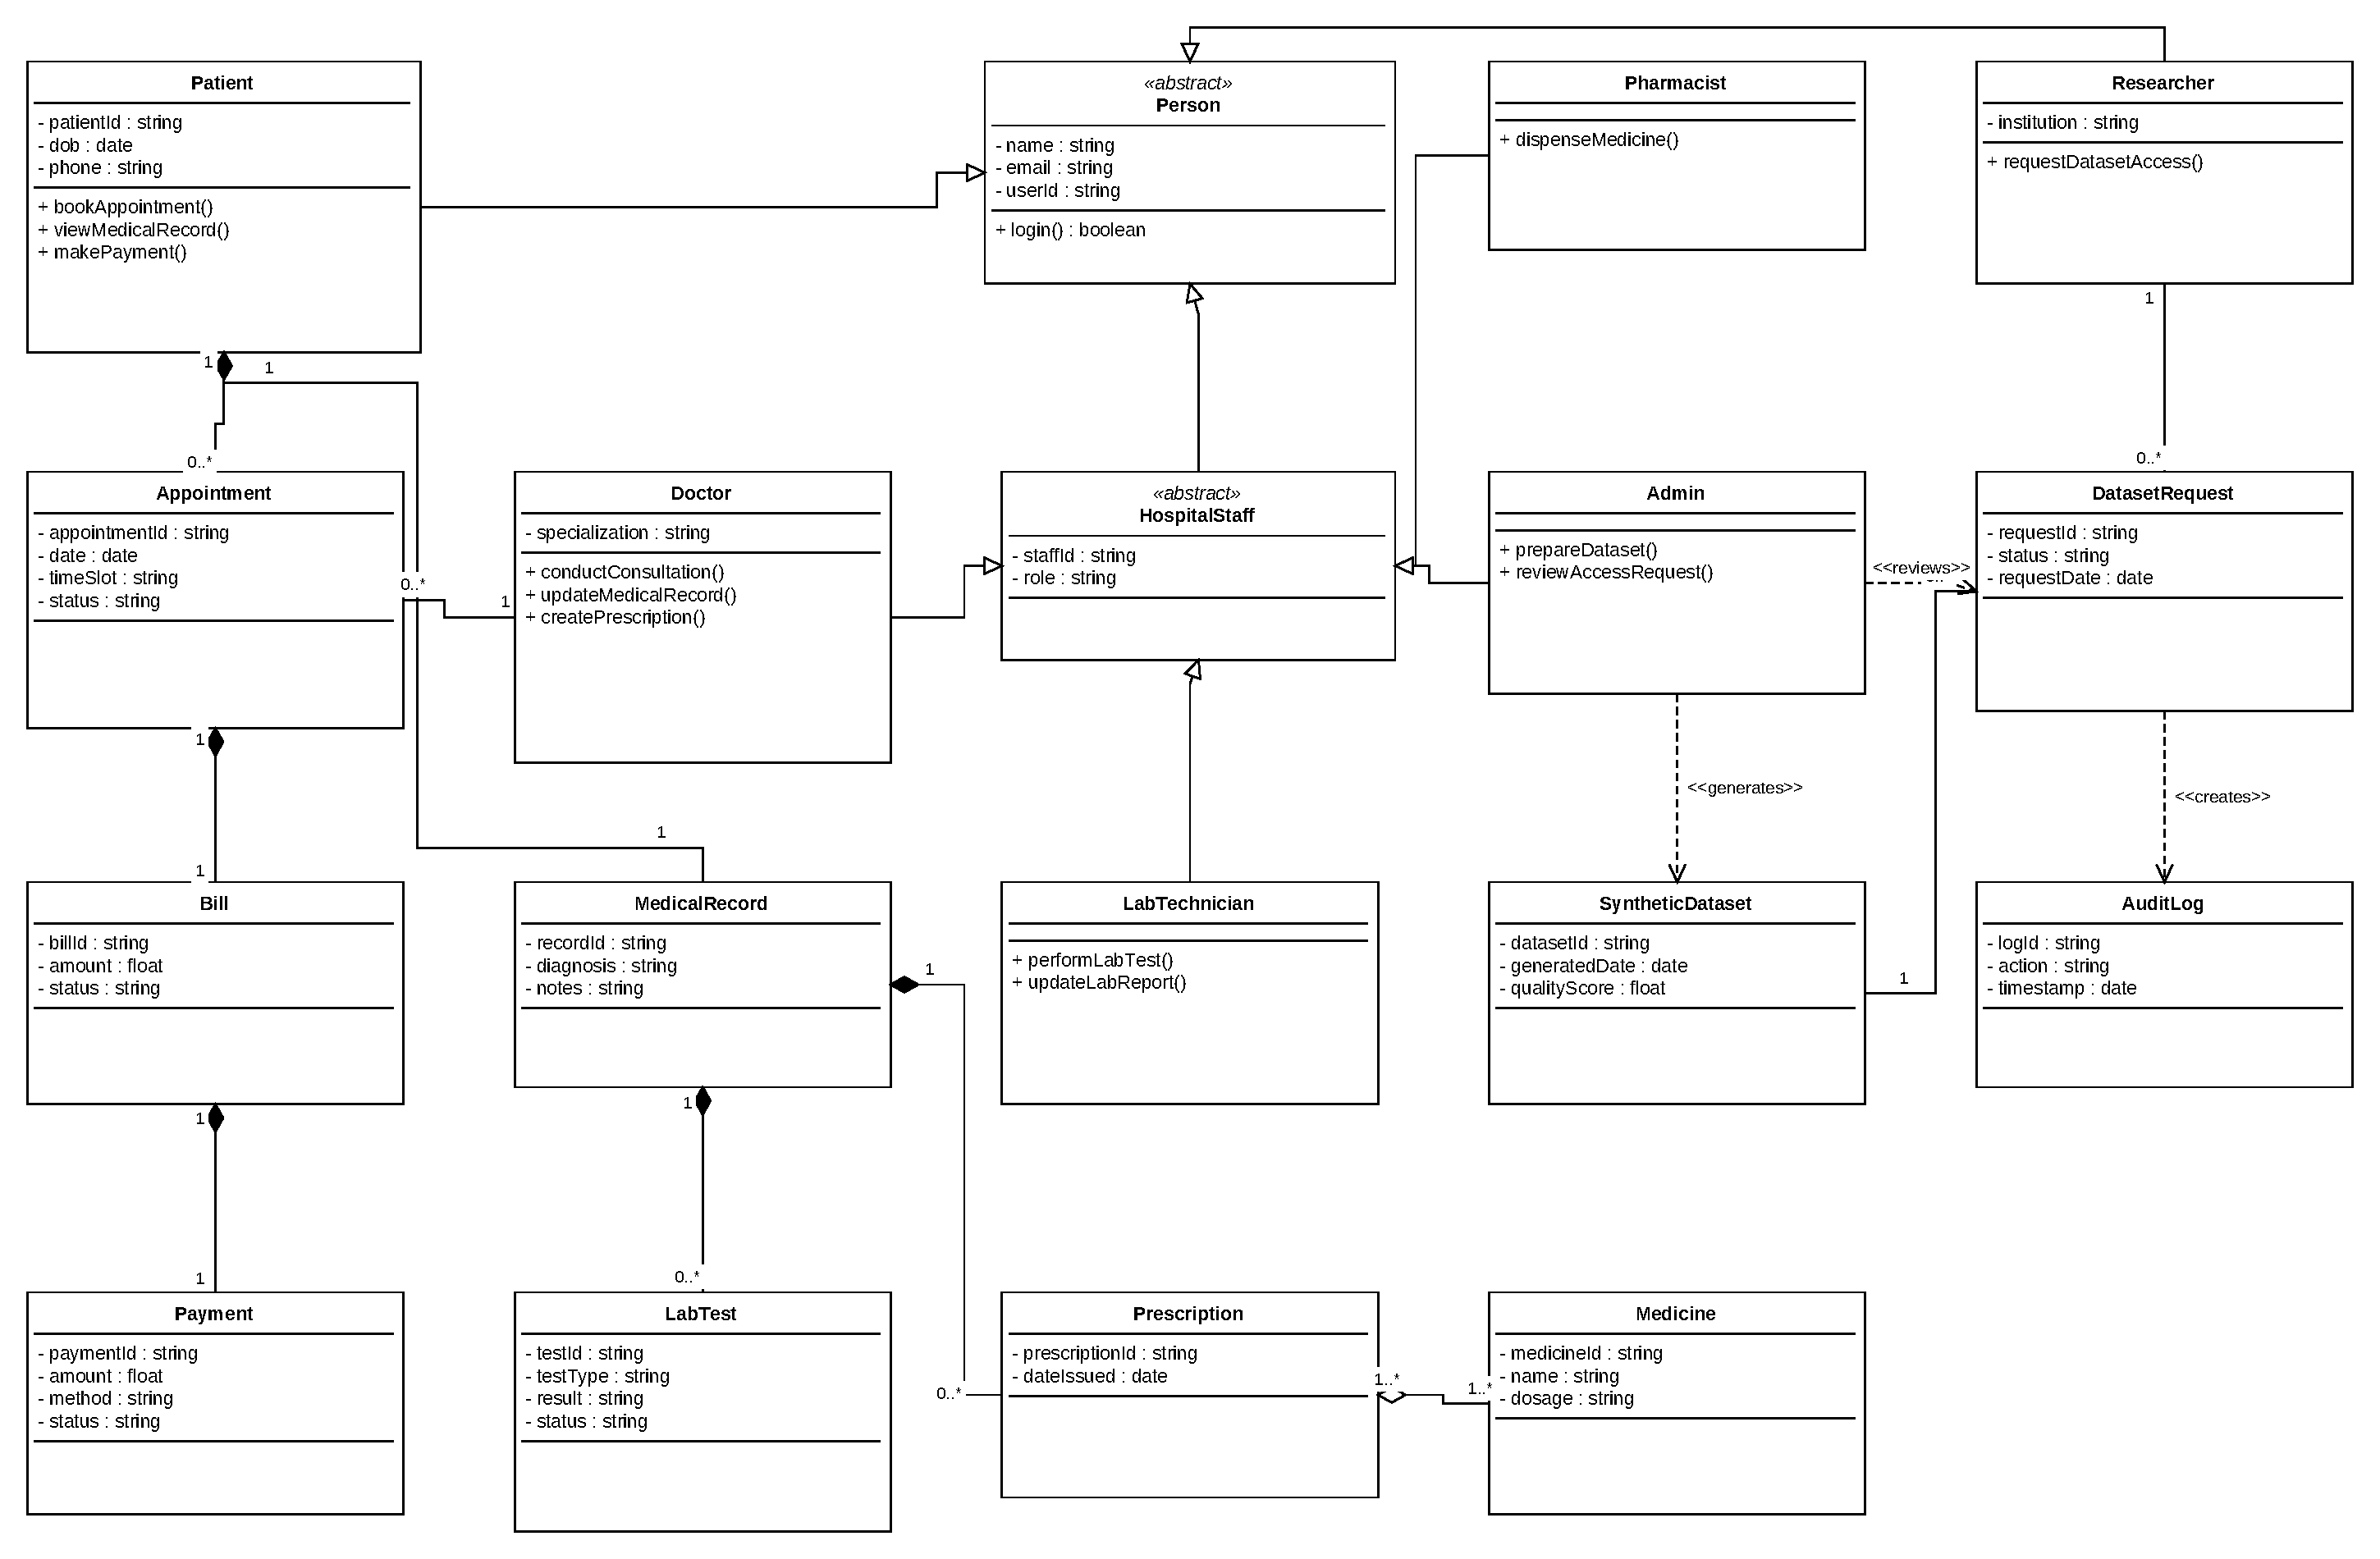
\includegraphics[width=\linewidth,height=0.82\textheight,keepaspectratio]{figures/class.pdf}
  \caption{Class diagram for MediSynth}
  \label{fig:class}
\end{figure}
\end{landscape}
\clearpage

% ----- Activity diagrams -----
\begin{landscape}
\section{Activity Diagram: Patient / Hospital Workflow}
\begin{figure}[H]
  \centering
  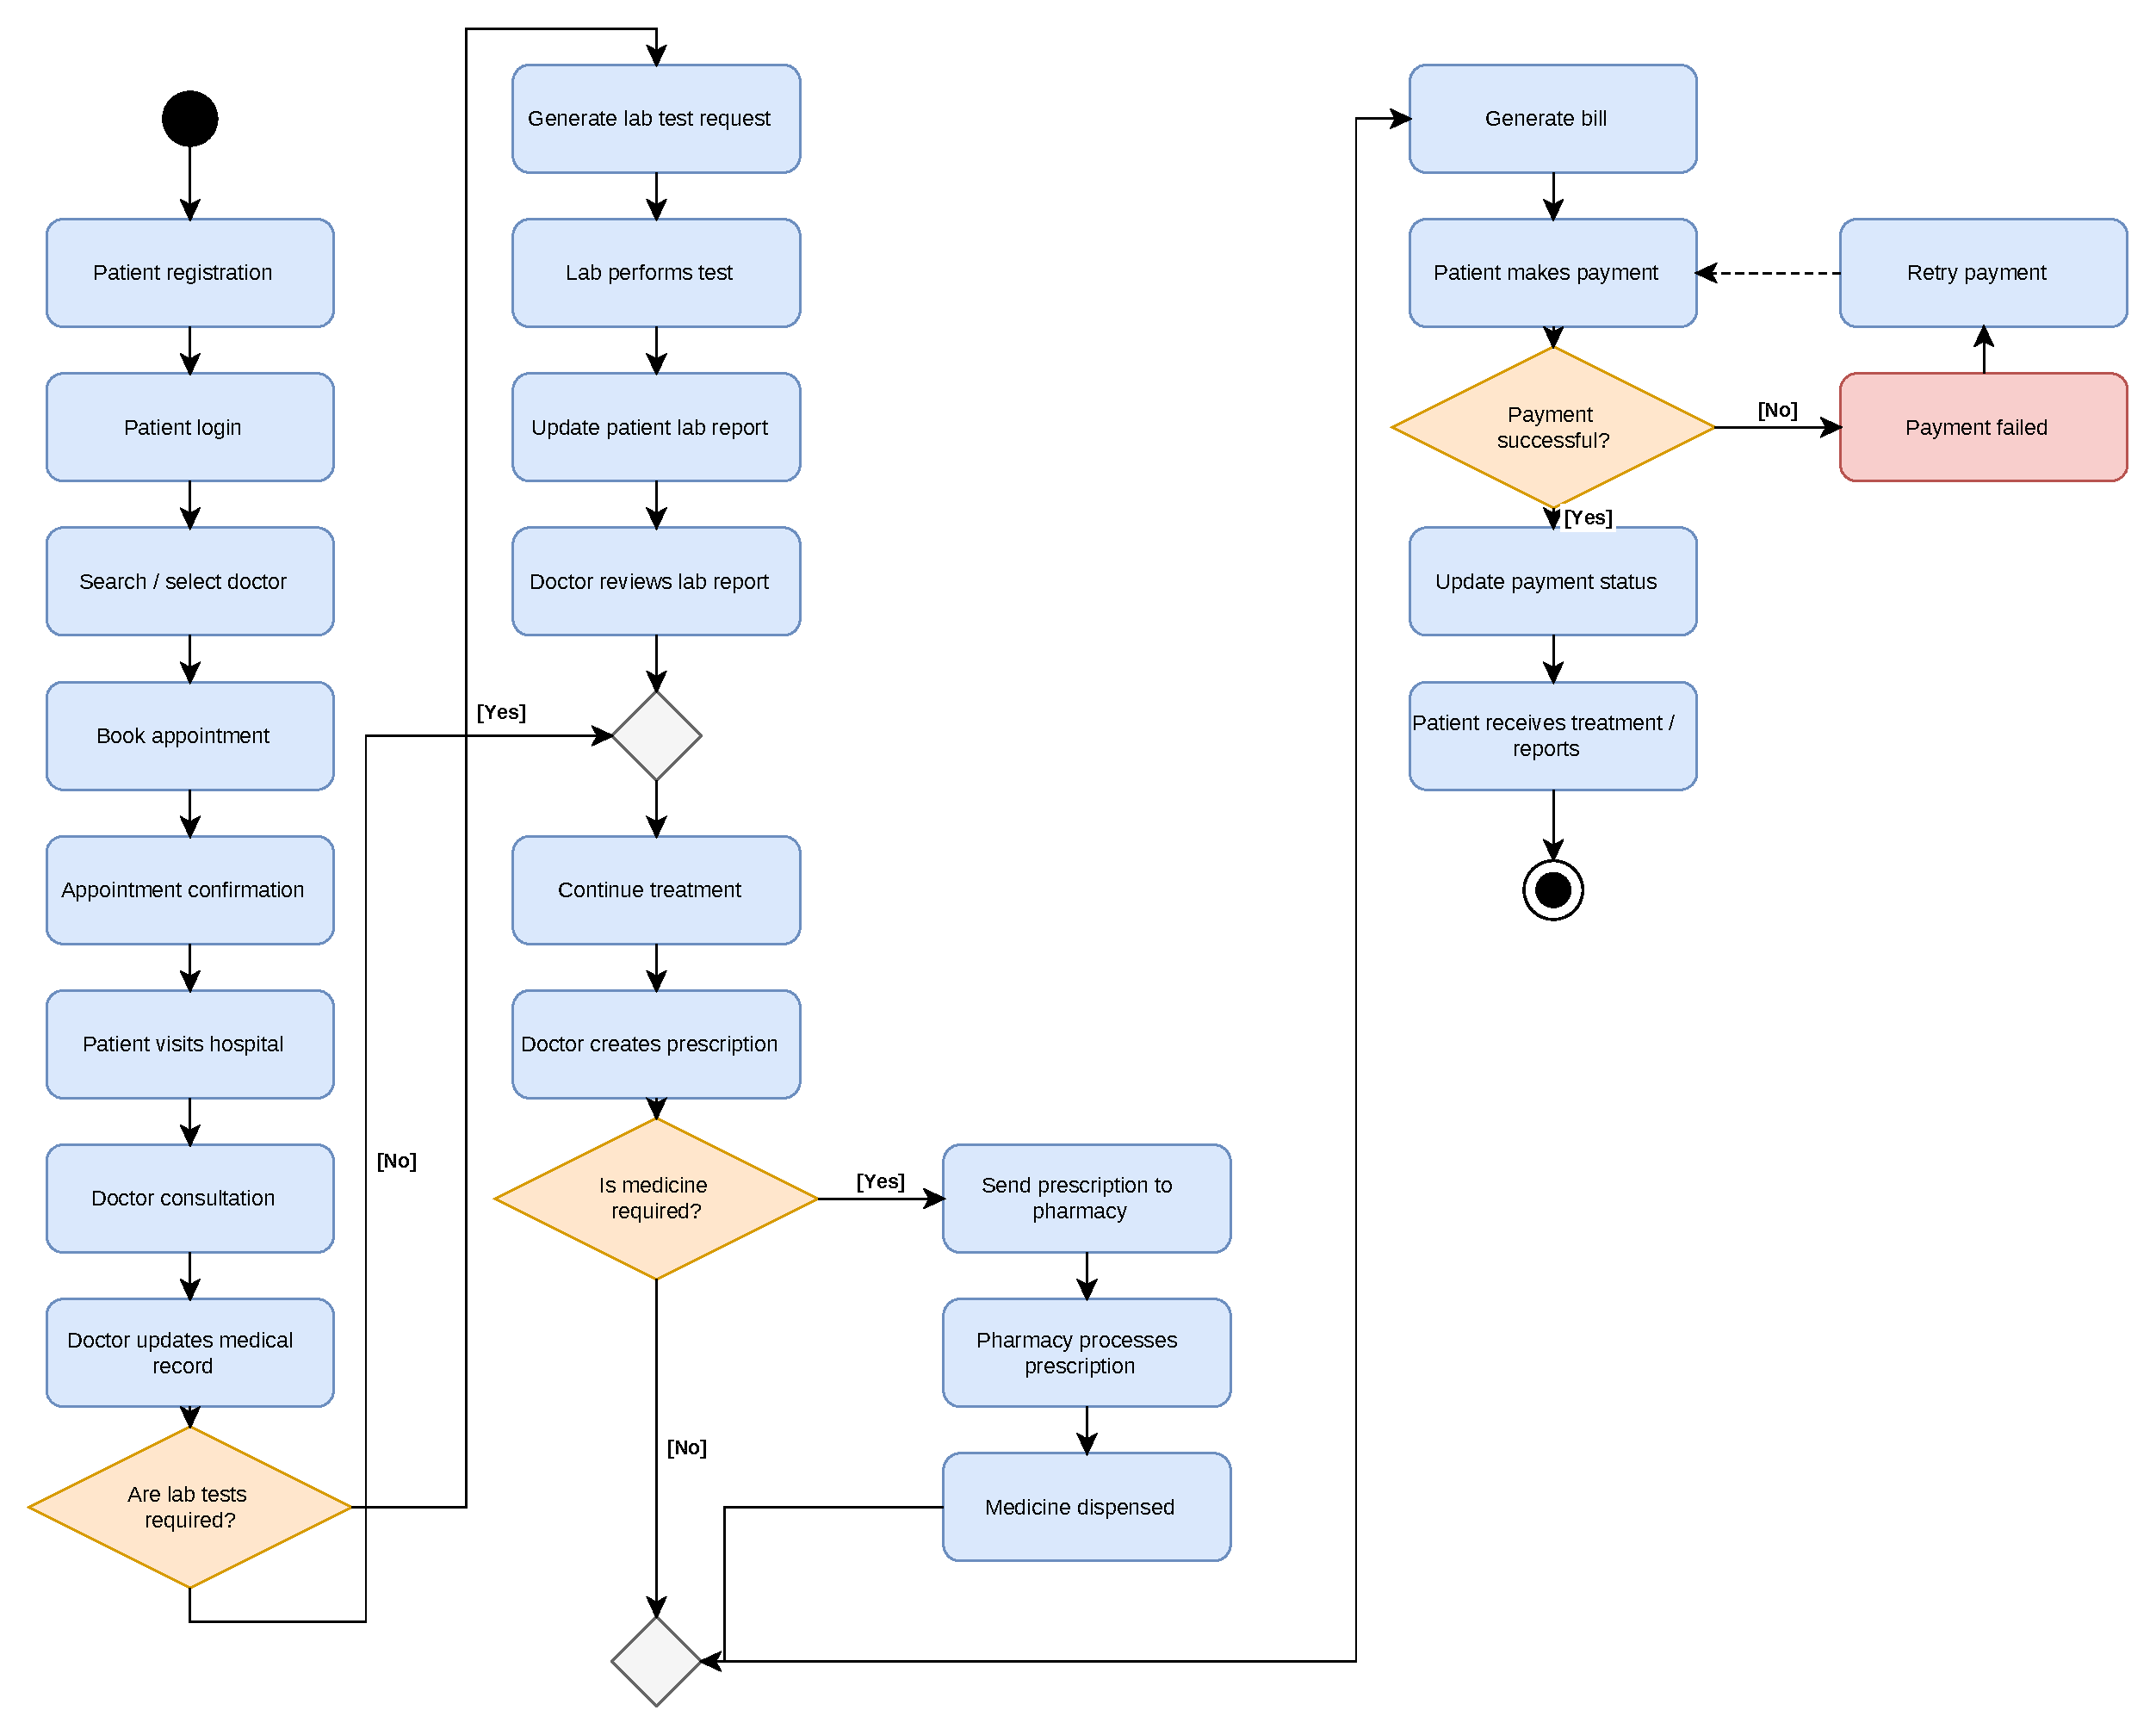
\includegraphics[width=\linewidth,height=0.82\textheight,keepaspectratio]{figures/activity1.pdf}
  \caption{Activity diagram: patient / hospital workflow}
  \label{fig:activity1}
\end{figure}
\end{landscape}
\clearpage

\section{Activity Diagram: Synthetix Workflow}

This workflow begins once sufficient patient / medical
record data has been accumulated by the hospital
workflow.

\begin{figure}[H]
  \centering
  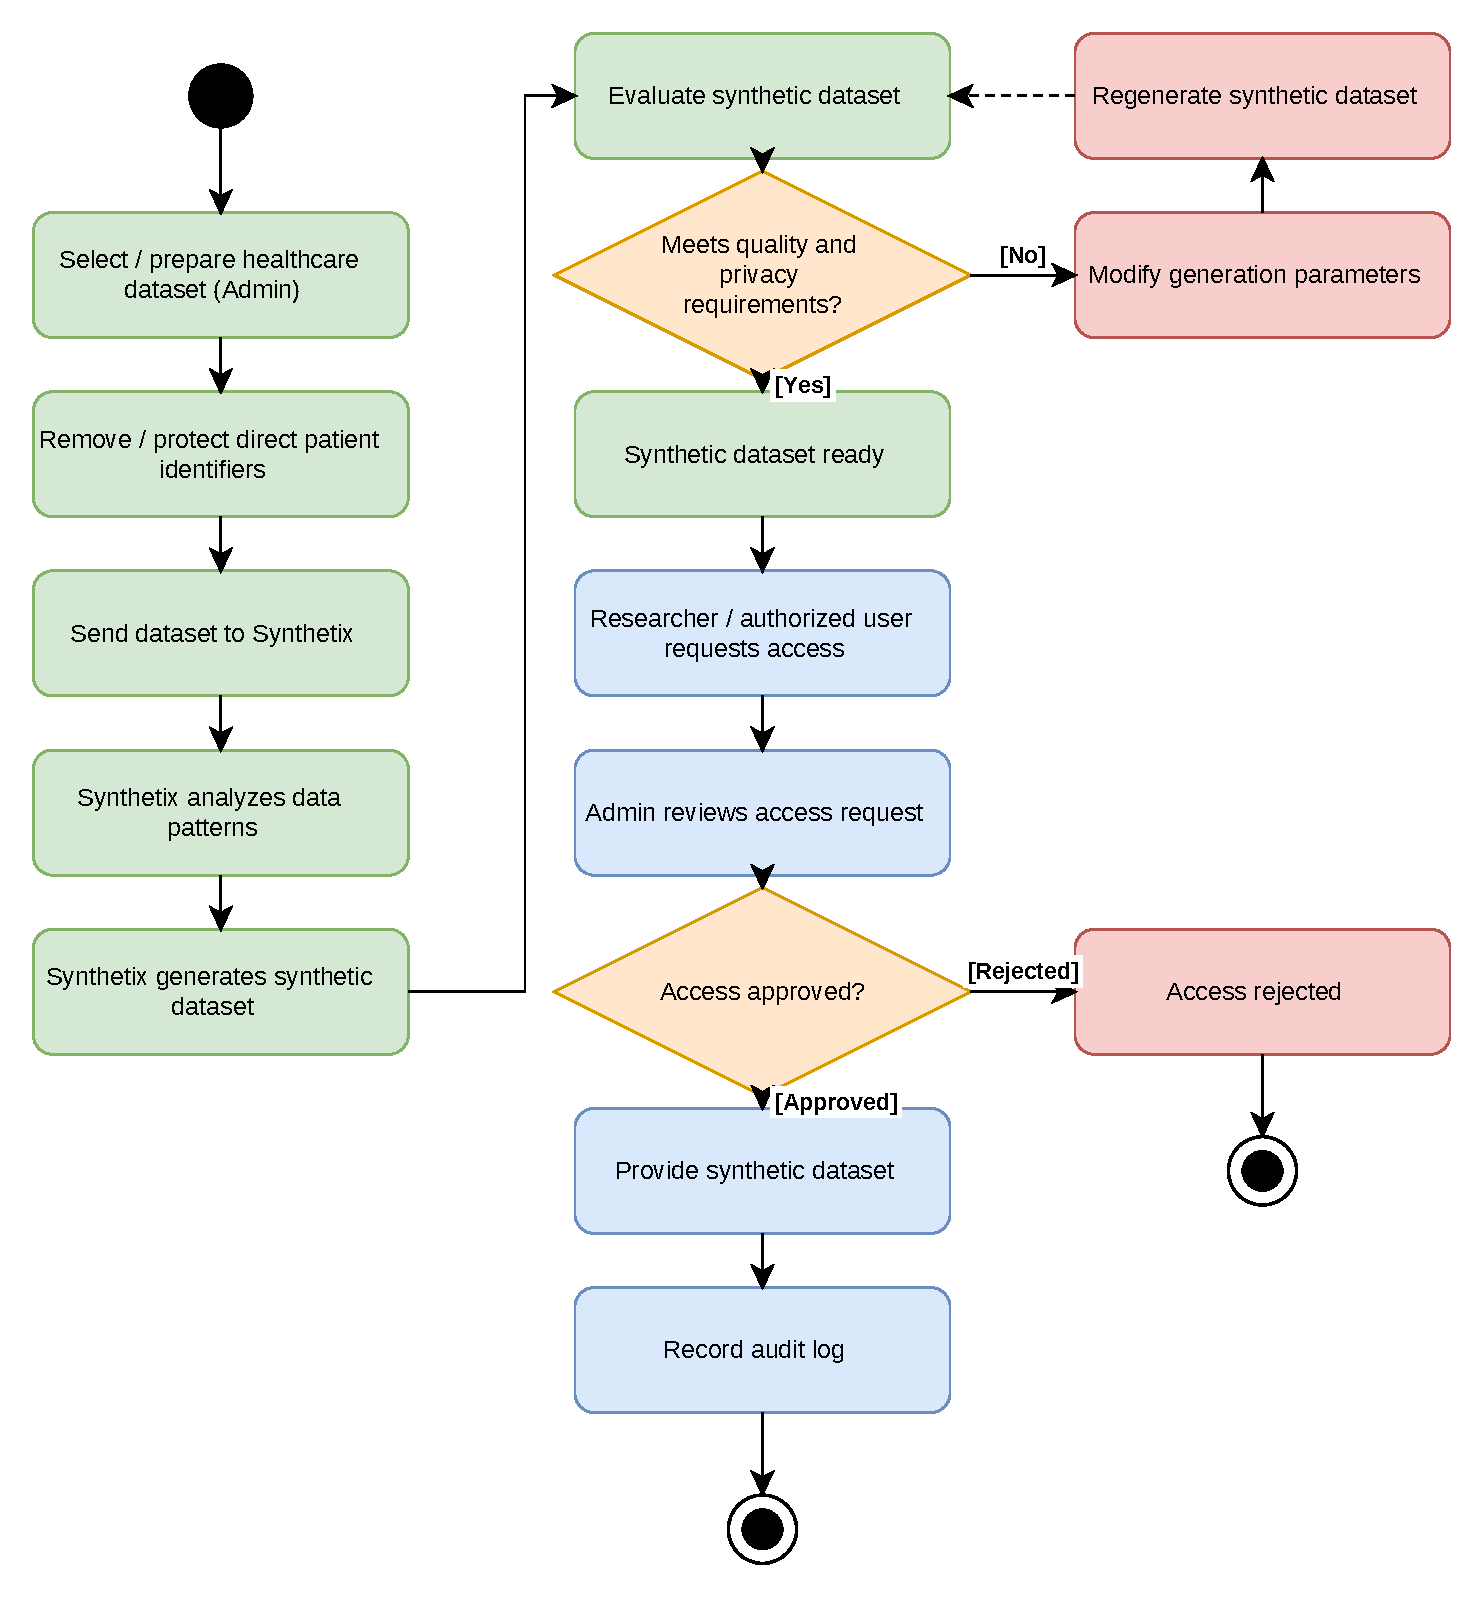
\includegraphics[width=\textwidth,height=0.66\textheight,keepaspectratio]{figures/activity2.pdf}
  \caption{Activity diagram: Synthetix workflow}
  \label{fig:activity2}
\end{figure}
\clearpage

% ----- Swimlane diagrams -----
\section{Swimlane Diagram 1: Patient / Hospital Workflow}

\begin{figure}[H]
  \centering
  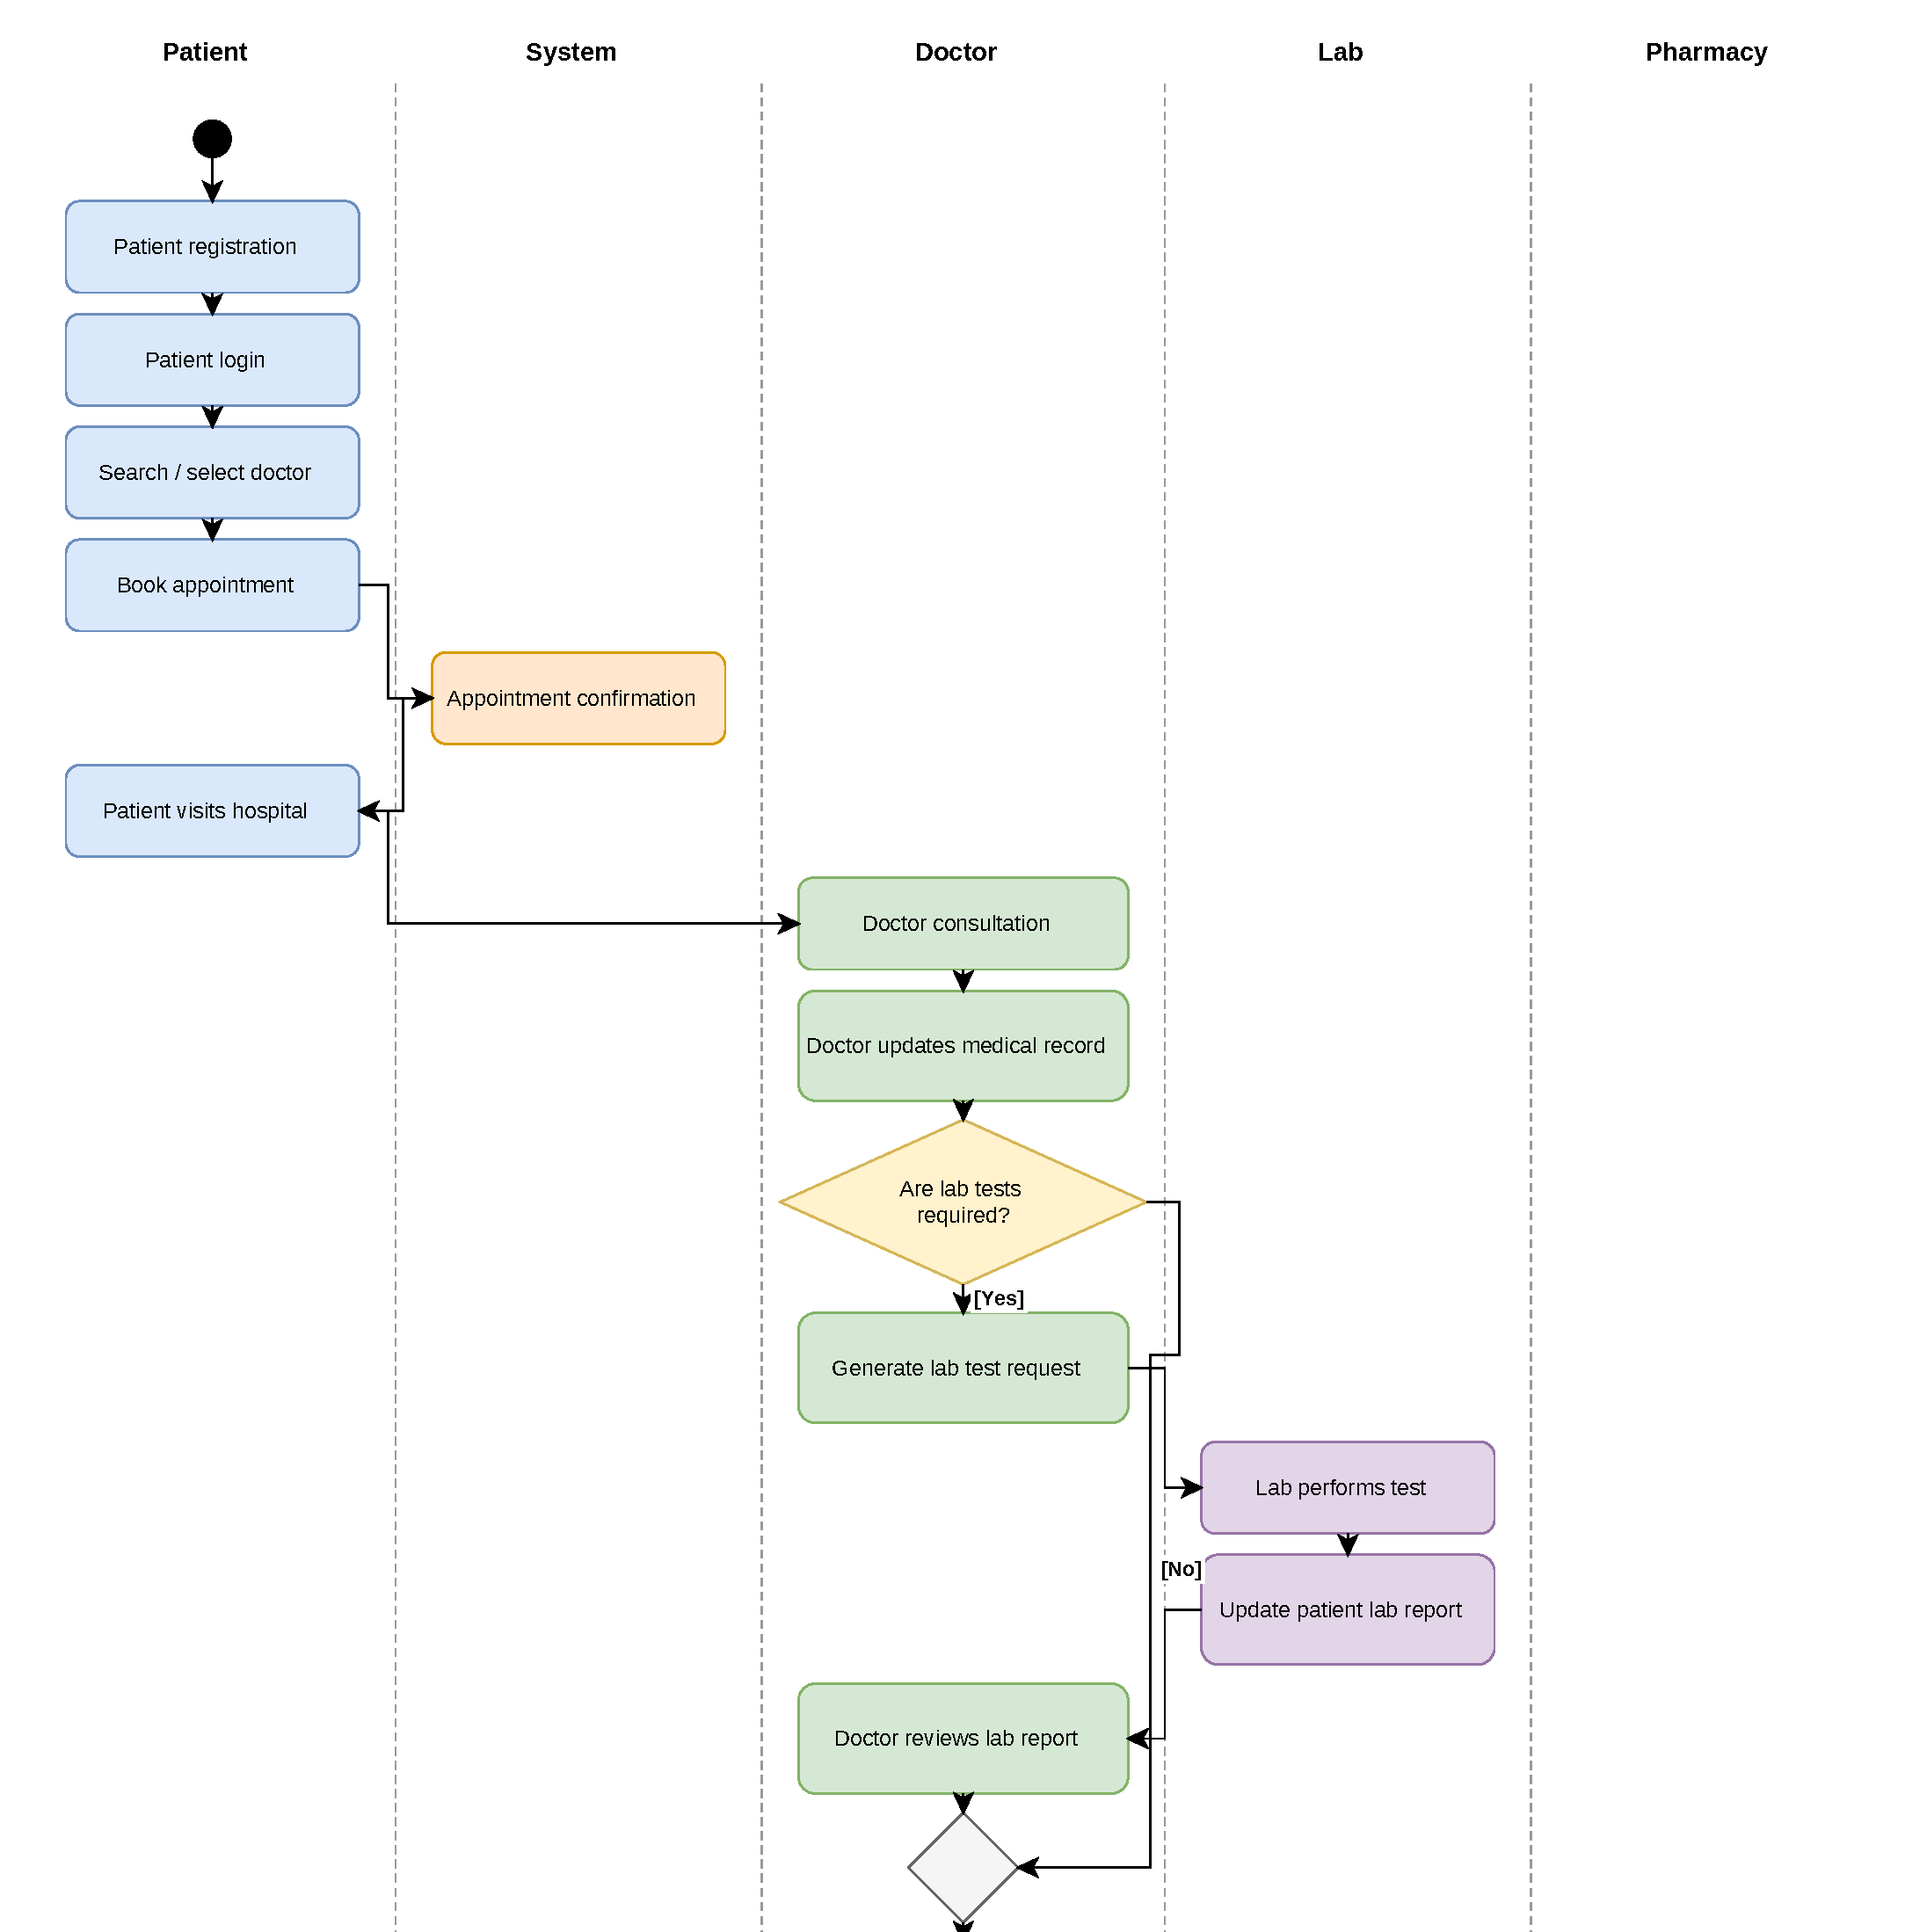
\includegraphics[width=\textwidth,height=0.72\textheight,keepaspectratio]{figures/swimlane1a.pdf}
  \caption{Swimlane diagram 1: patient / hospital workflow (part 1)}
  \label{fig:swimlane1a}
\end{figure}
\clearpage

\begin{figure}[H]
  \centering
  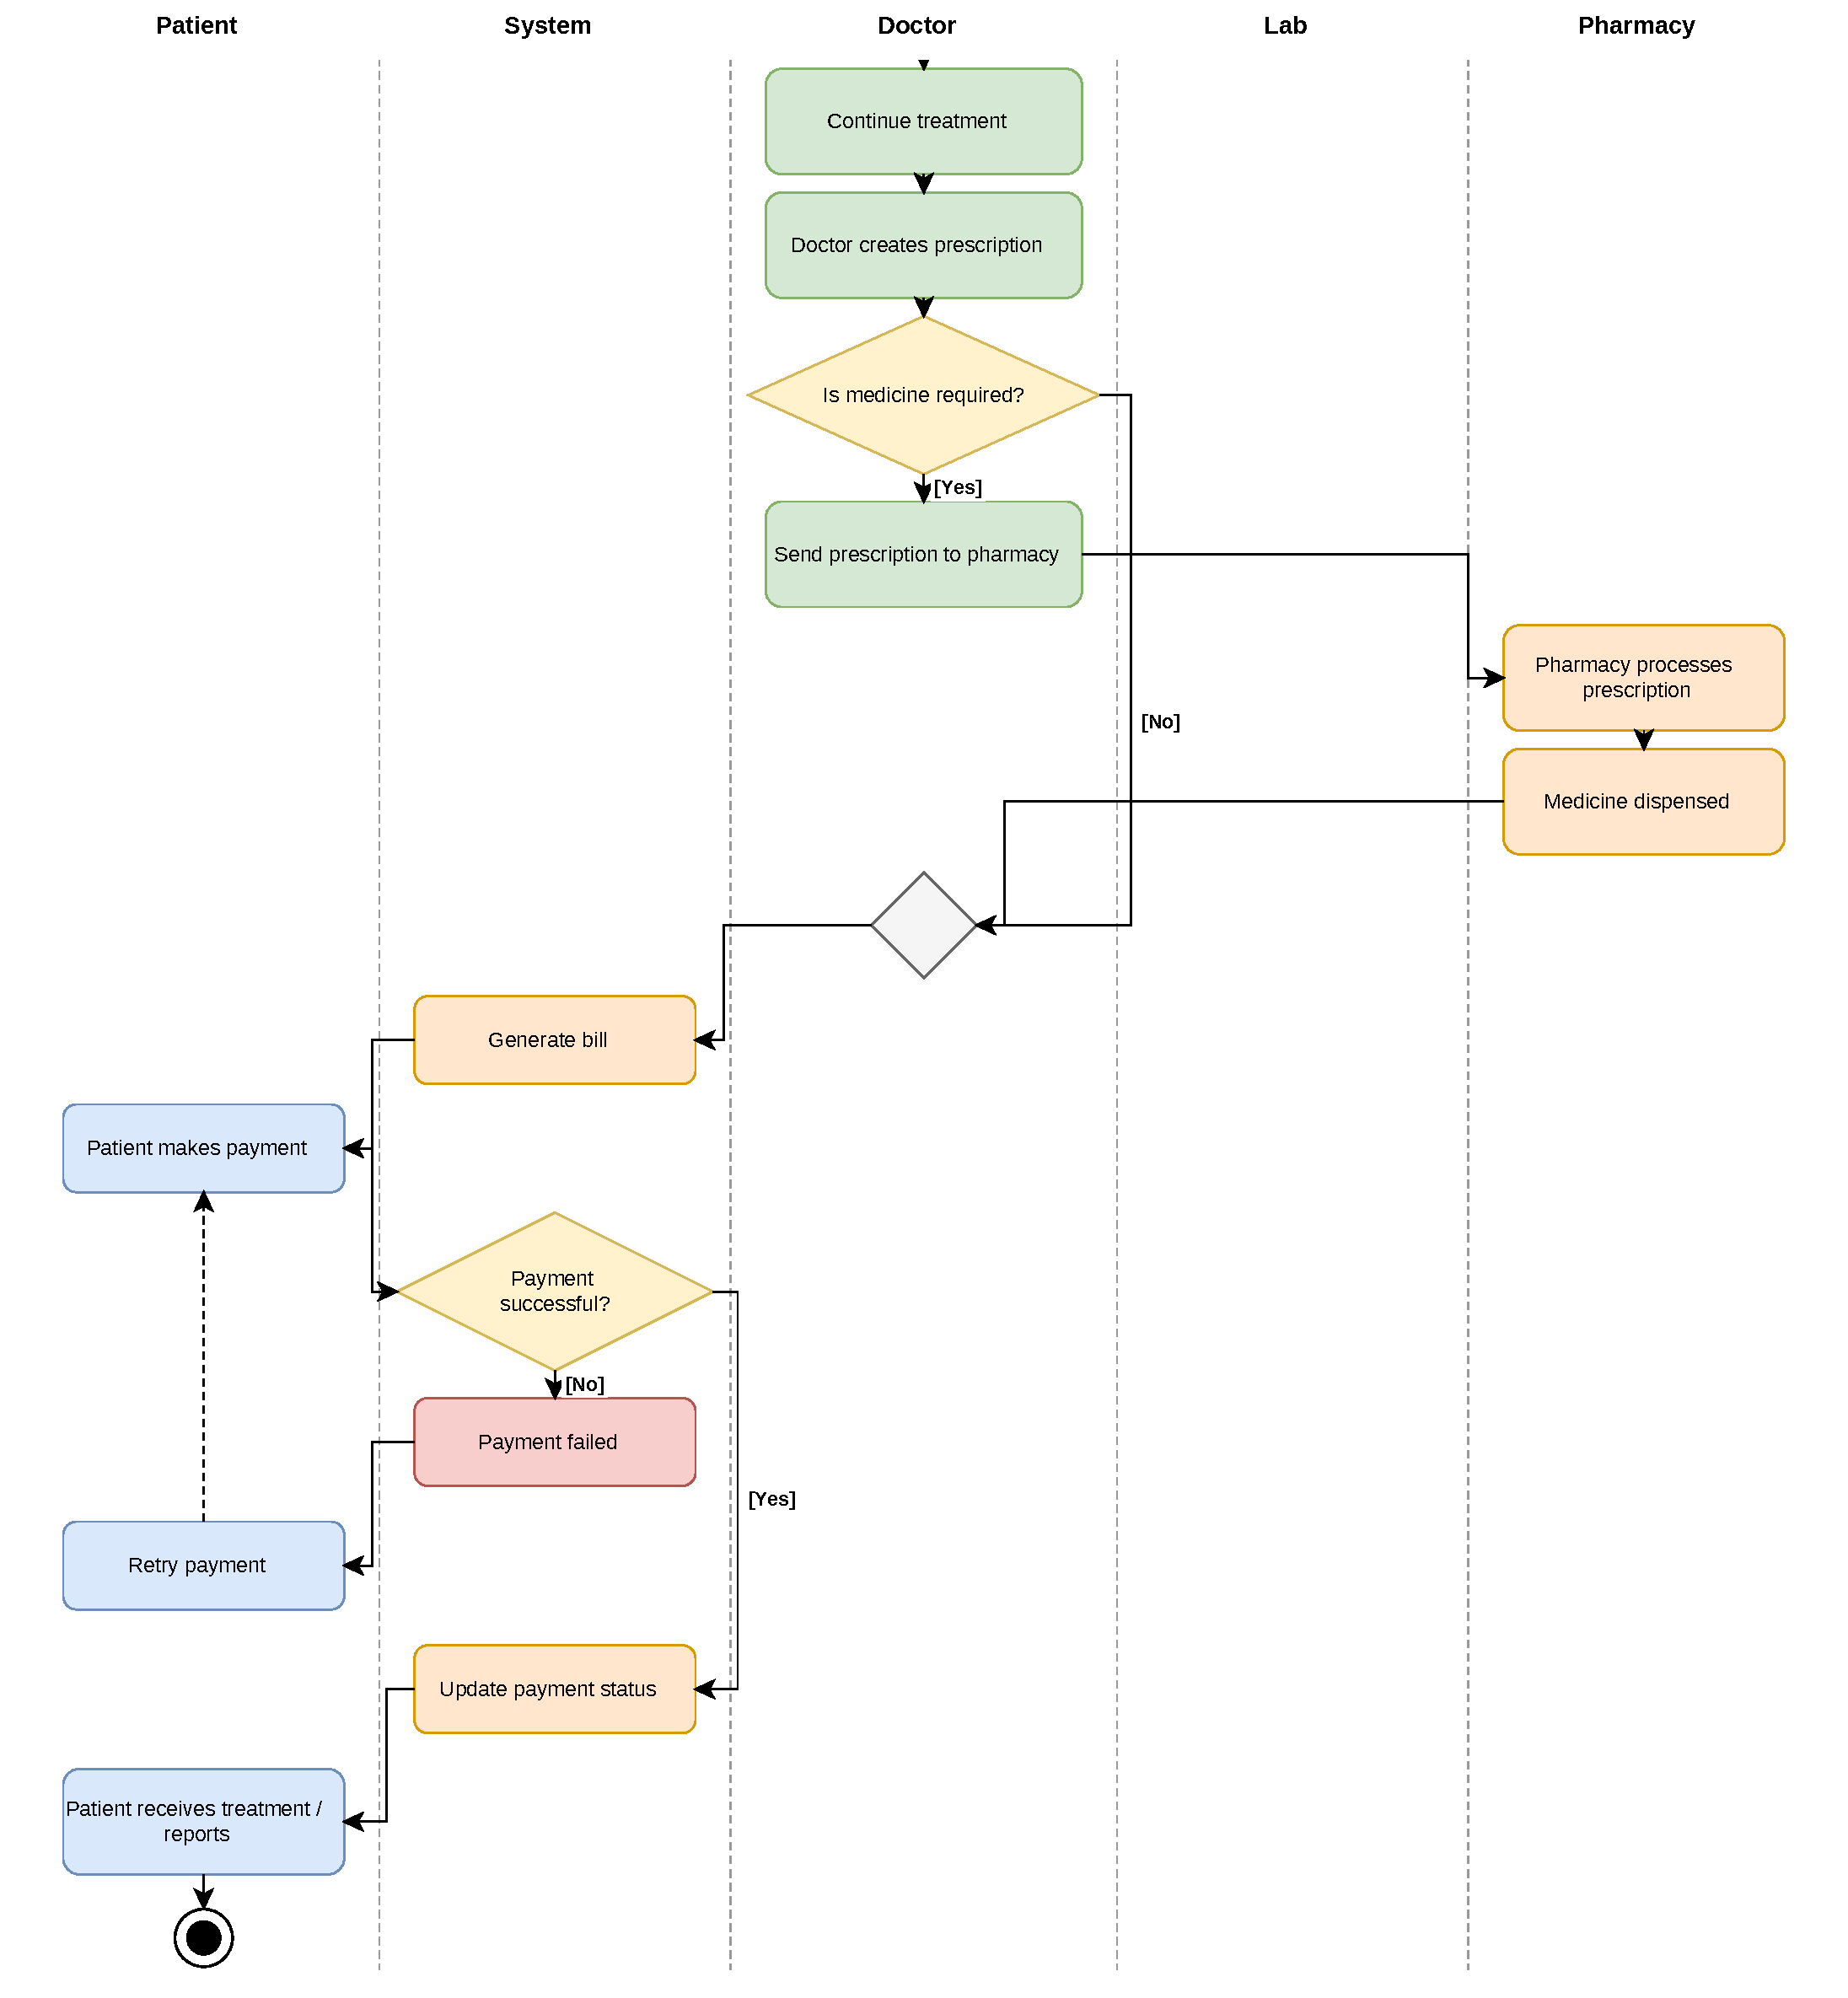
\includegraphics[width=\textwidth,height=0.72\textheight,keepaspectratio]{figures/swimlane1b.pdf}
  \caption{Swimlane diagram 1: patient / hospital workflow (part 2, continued)}
  \label{fig:swimlane1b}
\end{figure}
\clearpage

\section{Swimlane Diagram 2: Synthetix Workflow}

\begin{figure}[H]
  \centering
  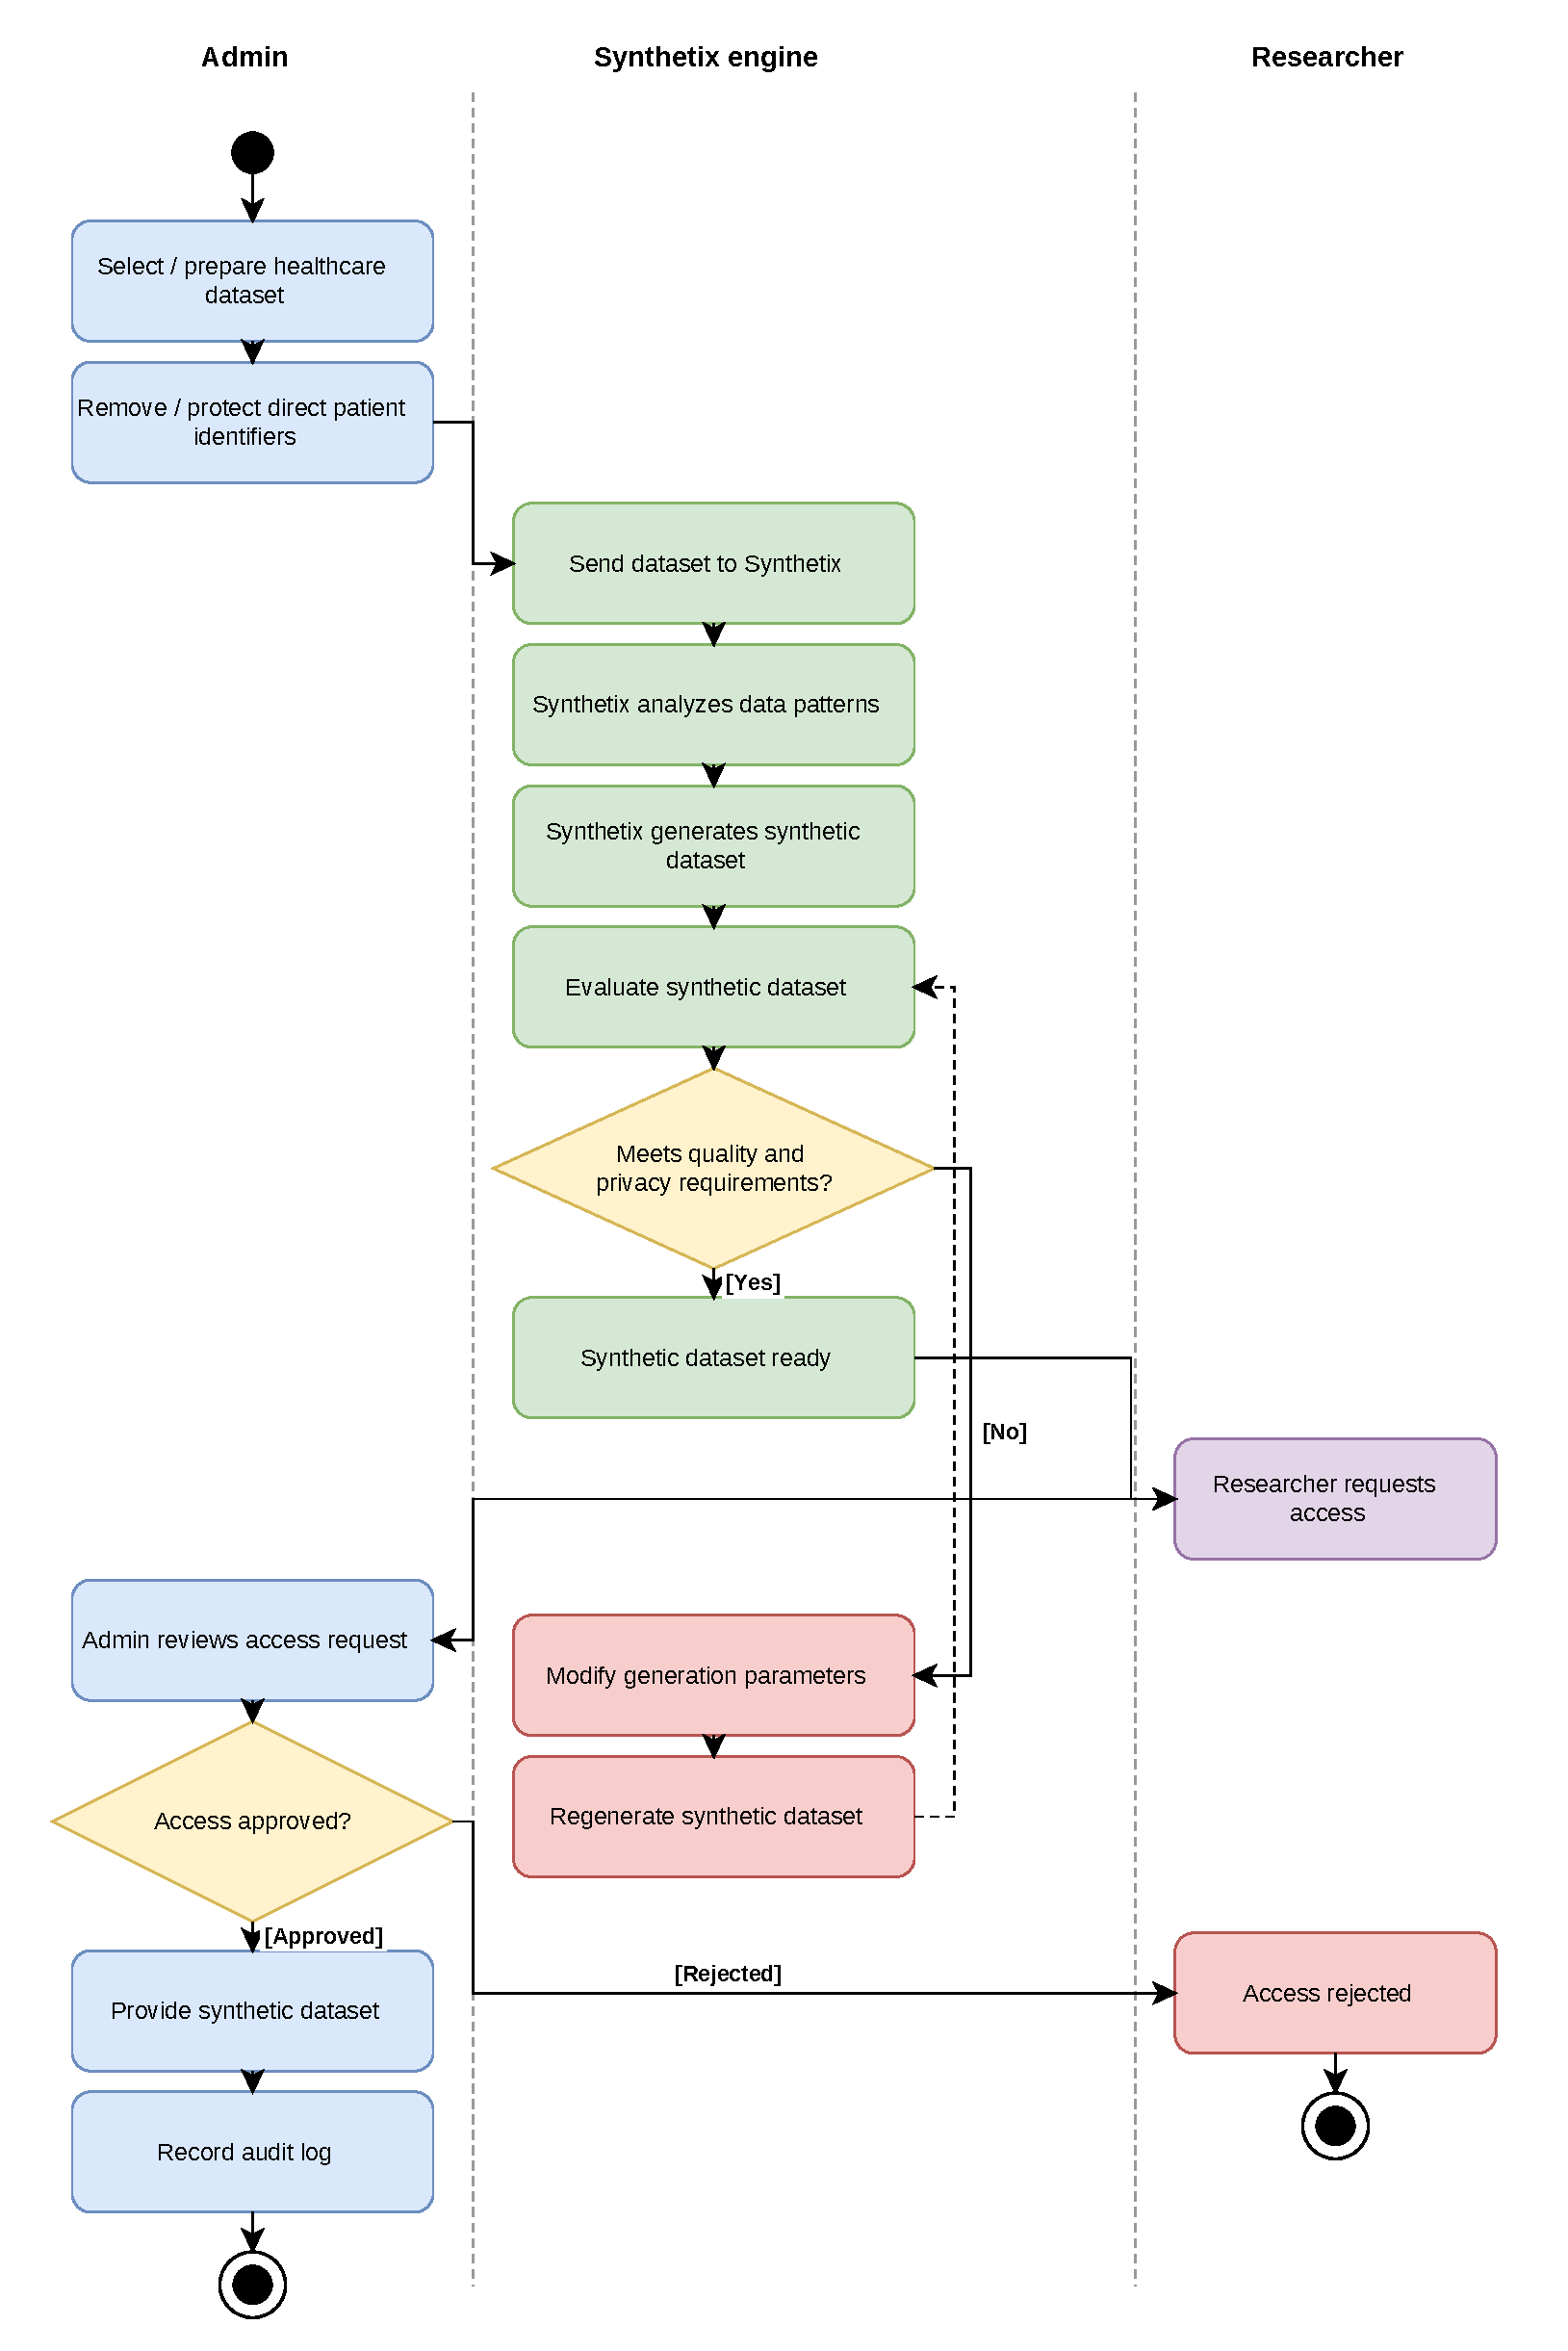
\includegraphics[width=\textwidth,height=0.72\textheight,keepaspectratio]{figures/swimlane2.pdf}
  \caption{Swimlane diagram 2: Synthetix workflow}
  \label{fig:swimlane2}
\end{figure}
\clearpage

% ----- Data flow diagrams -----
\begin{landscape}
\section{Data Flow Diagram: Level 0 (Context Diagram)}

\begin{figure}[H]
  \centering
  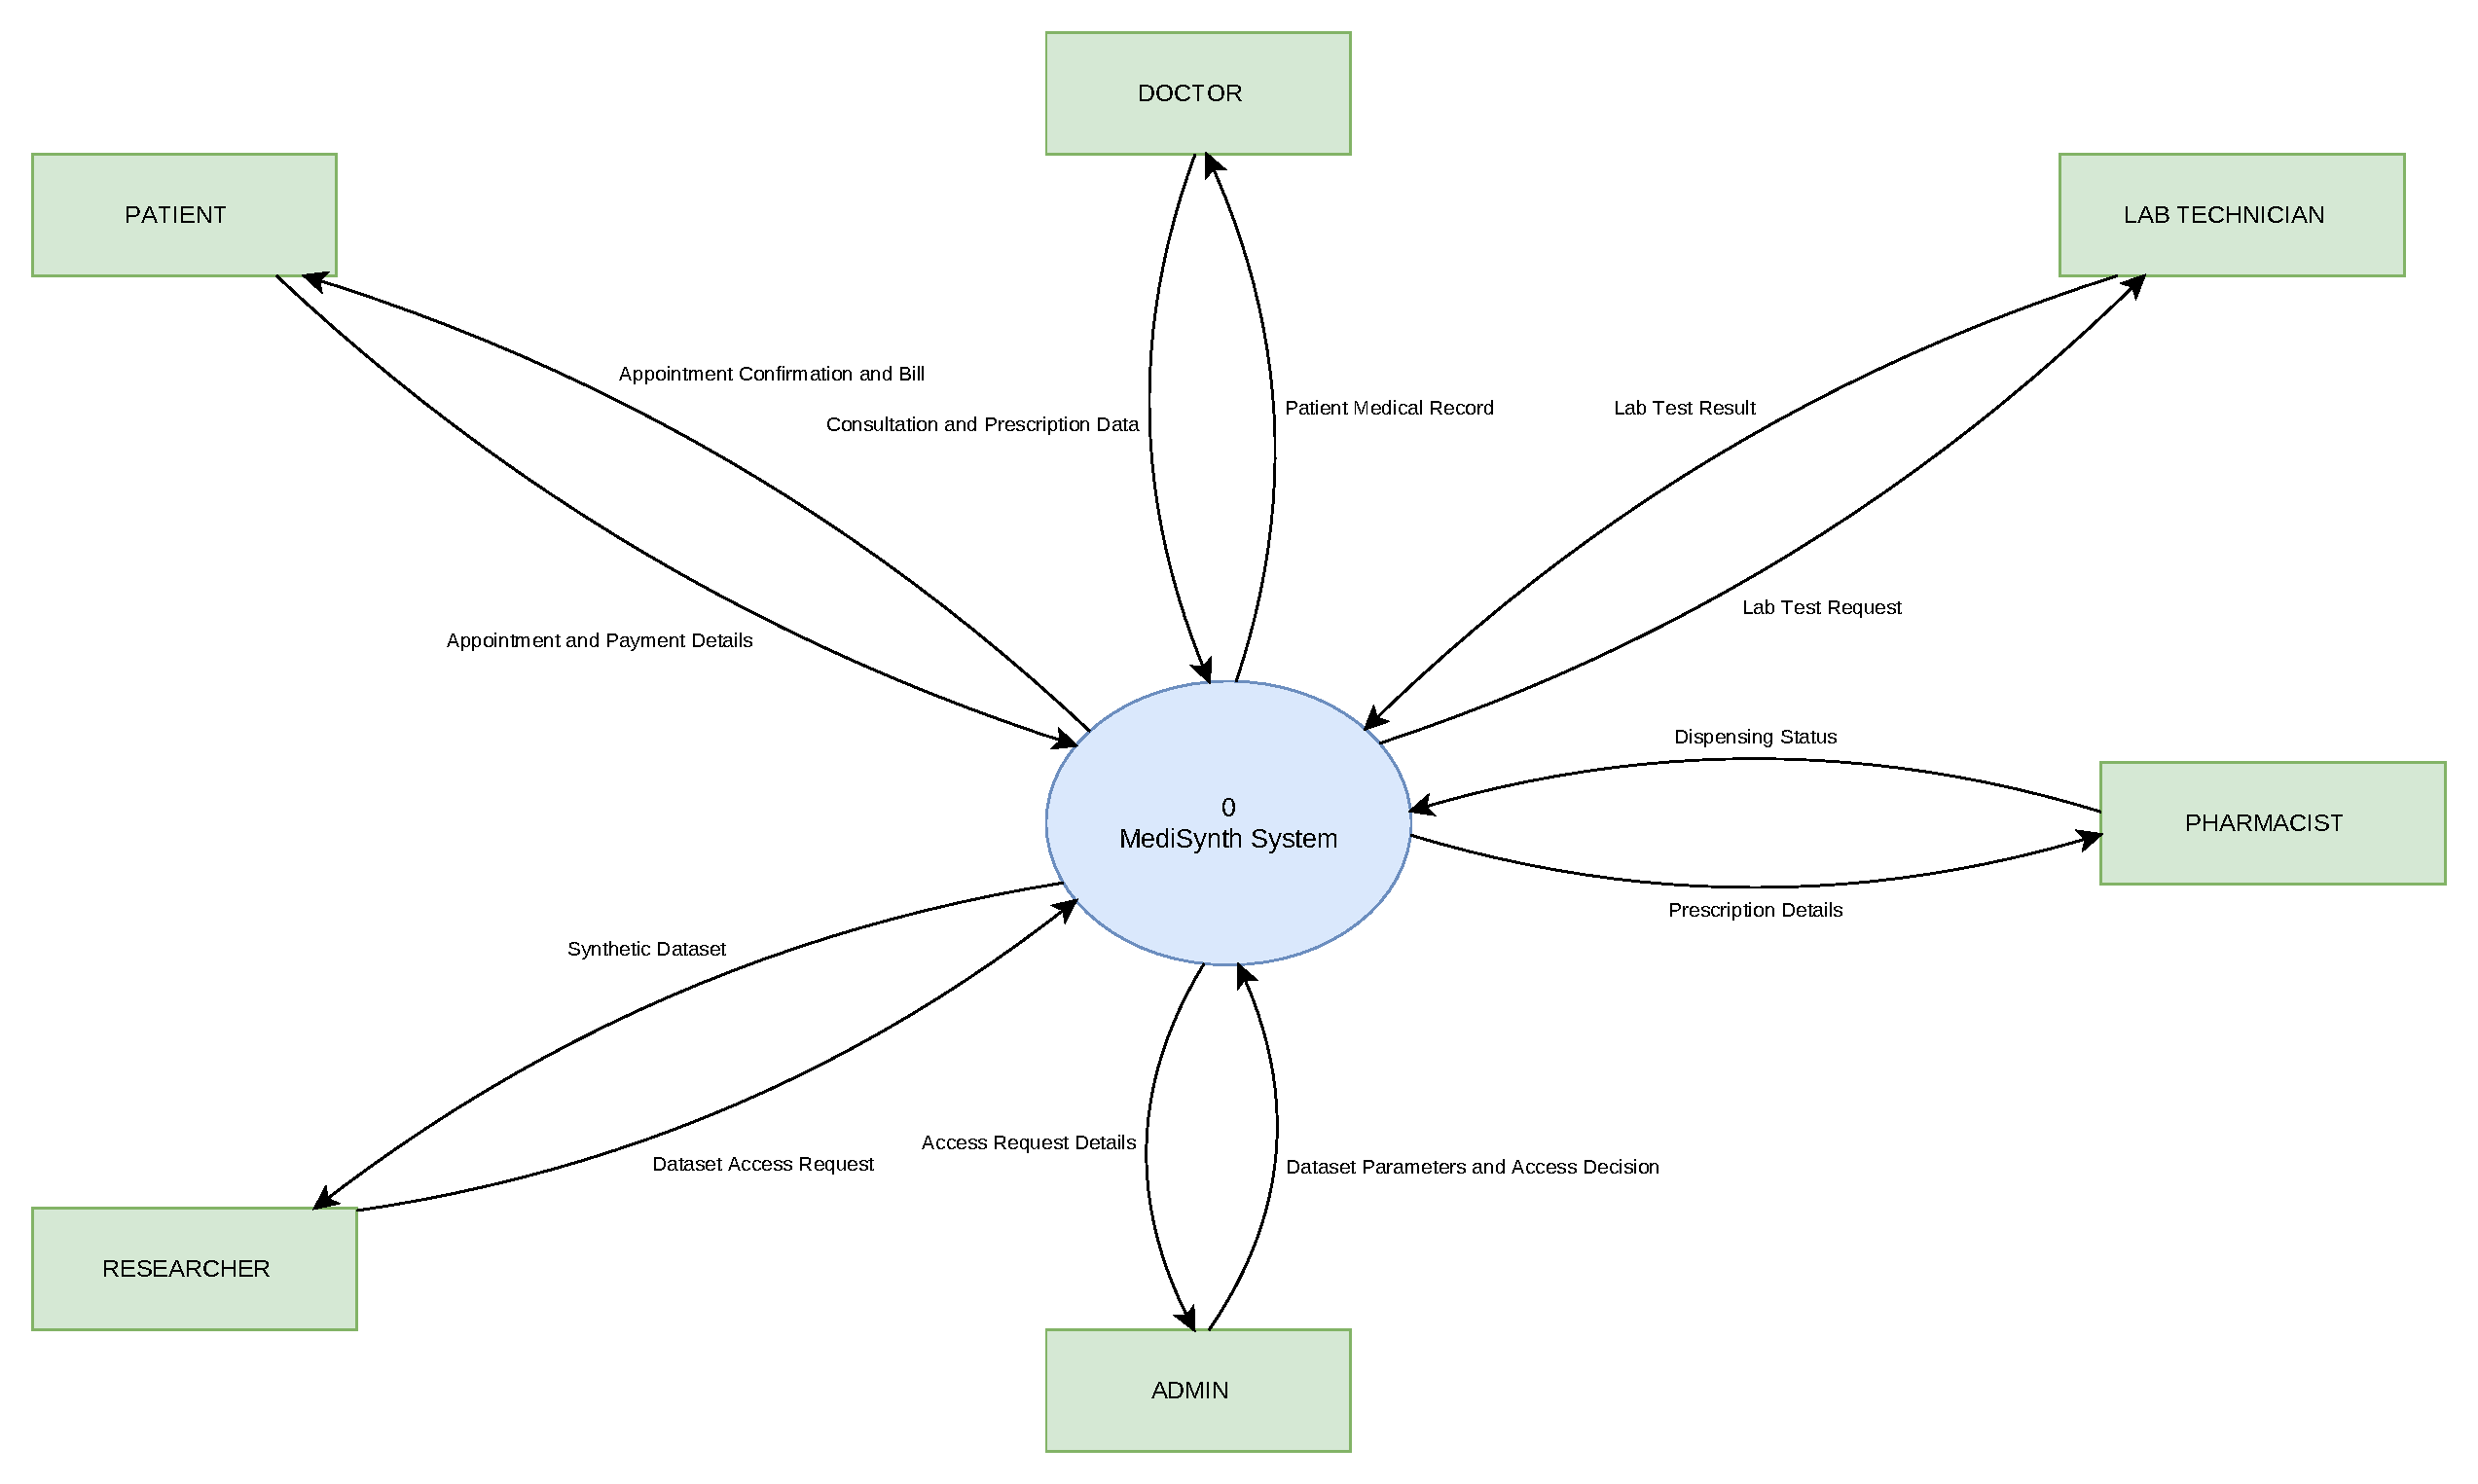
\includegraphics[width=\linewidth,height=0.82\textheight,keepaspectratio]{figures/dfd0.pdf}
  \caption{Data flow diagram: level 0 (context diagram)}
  \label{fig:dfd0}
\end{figure}
\end{landscape}
\clearpage

\begin{landscape}
\section{Data Flow Diagram: Level 1}
\begin{figure}[H]
  \centering
  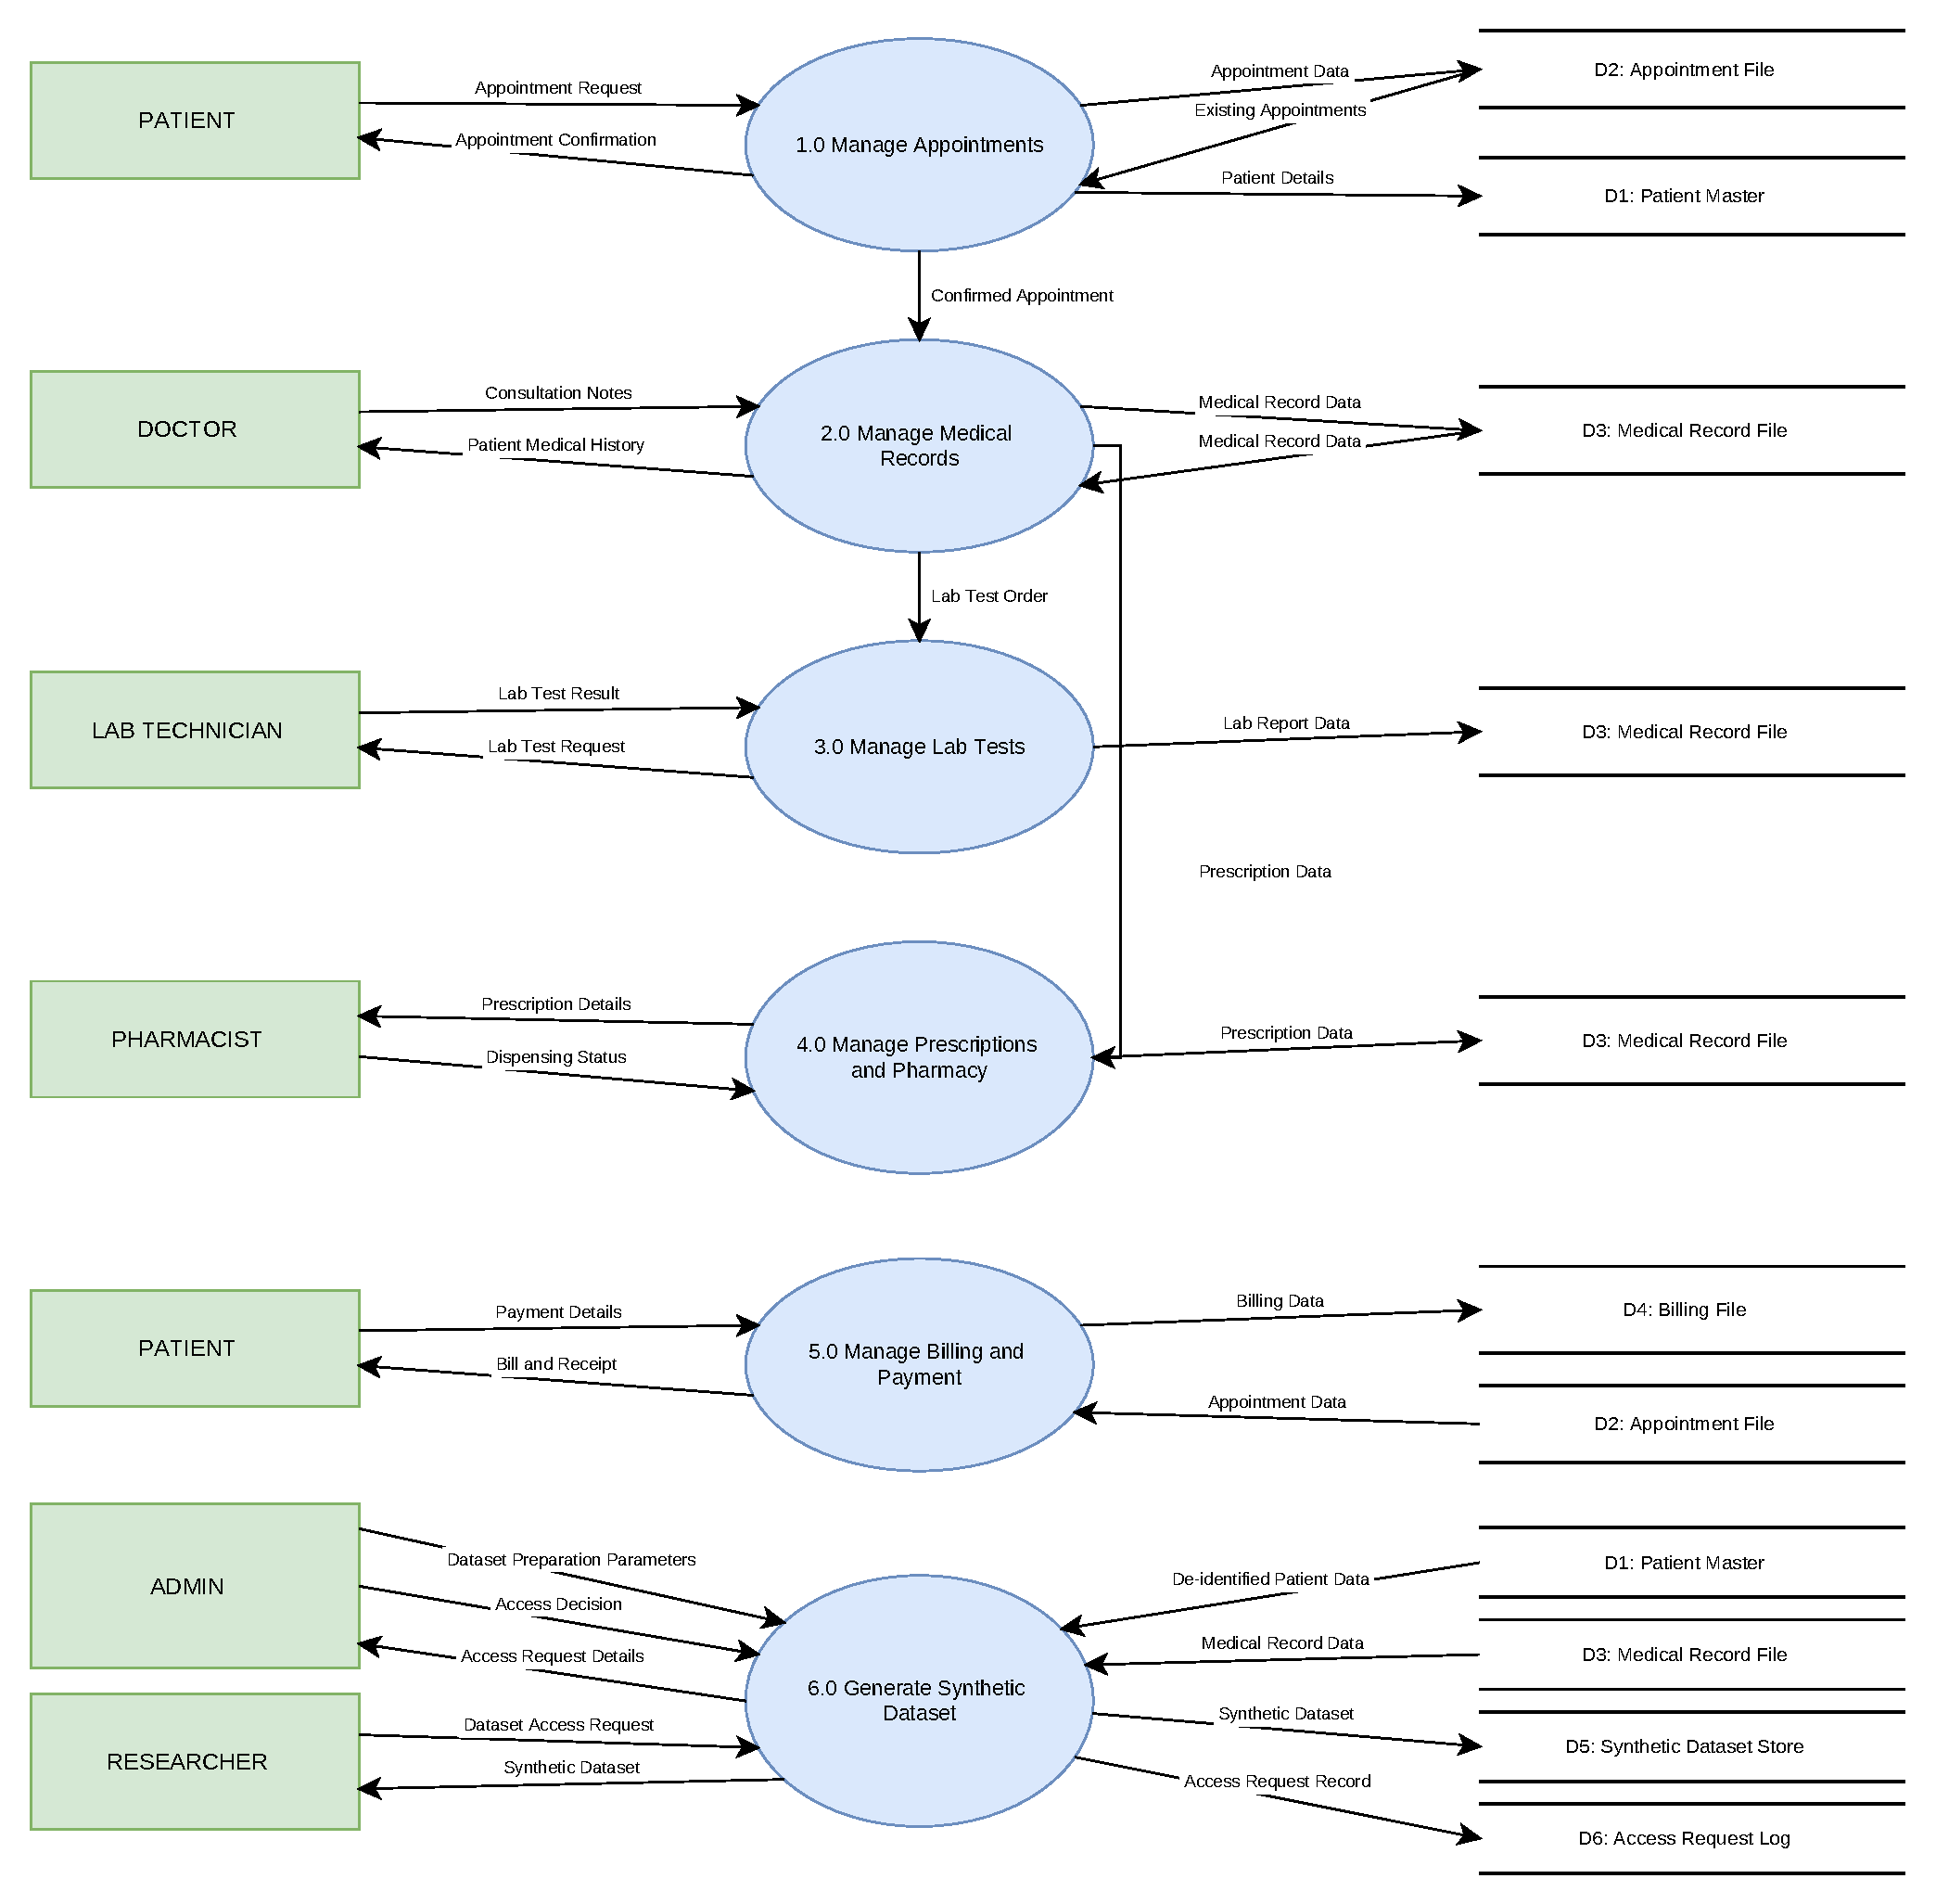
\includegraphics[width=\linewidth,height=0.82\textheight,keepaspectratio]{figures/dfd1.pdf}
  \caption{Data flow diagram: level 1}
  \label{fig:dfd1}
\end{figure}
\end{landscape}
\clearpage

% ----- Sequence diagrams -----
\section{Sequence Diagram 1: Book Appointment}

\begin{figure}[H]
  \centering
  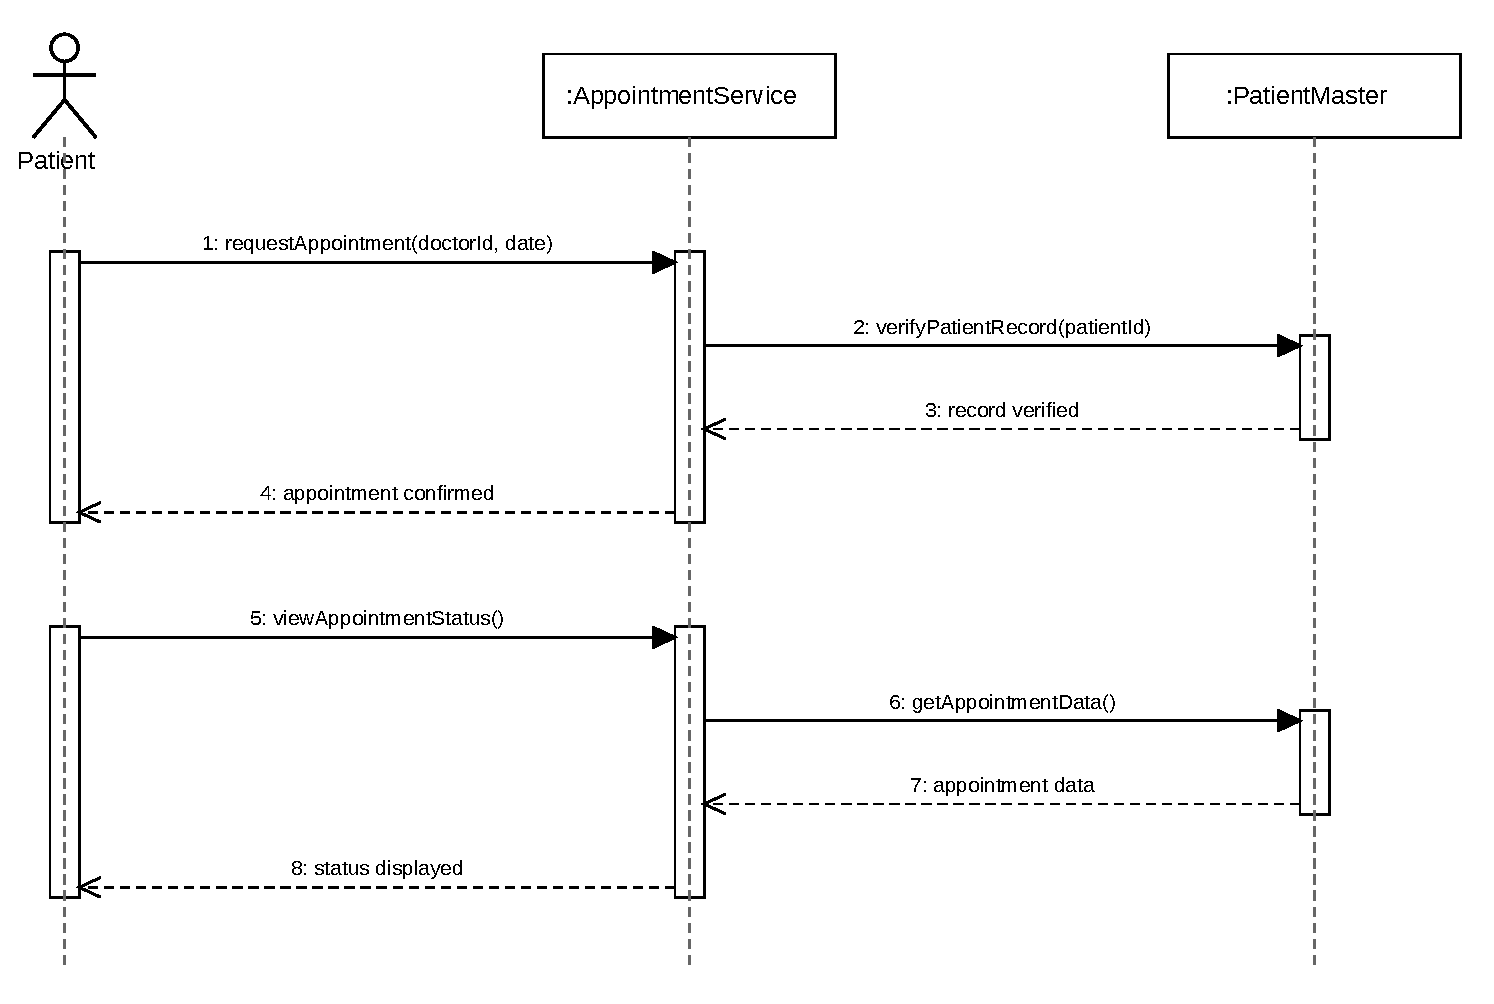
\includegraphics[width=\textwidth,height=0.72\textheight,keepaspectratio]{figures/seq1.pdf}
  \caption{Sequence diagram 1: book appointment}
  \label{fig:seq1}
\end{figure}
\clearpage

\begin{landscape}
\section{Sequence Diagram 2: Generate Synthetic Dataset}

\begin{figure}[H]
  \centering
  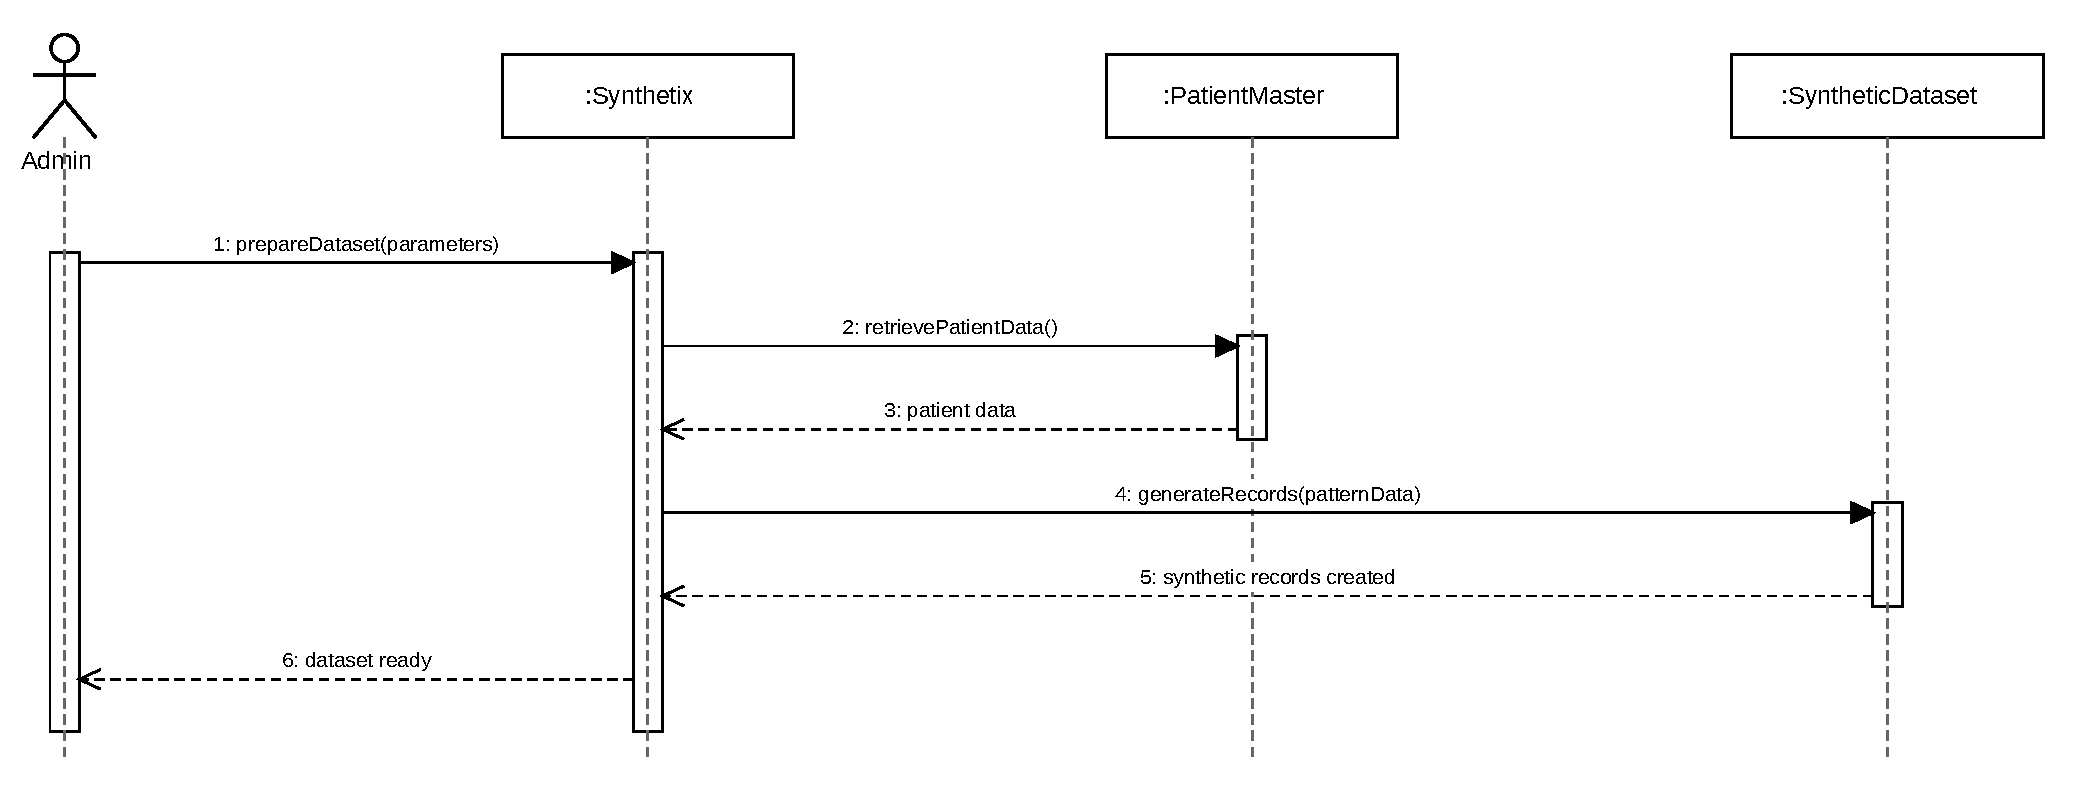
\includegraphics[width=\linewidth,height=0.82\textheight,keepaspectratio]{figures/seq2.pdf}
  \caption{Sequence diagram 2: generate synthetic dataset}
  \label{fig:seq2}
\end{figure}
\end{landscape}
\clearpage

% ----- Collaboration diagrams -----
\begin{landscape}
\section{Collaboration Diagram 1: Book Appointment}

\begin{figure}[H]
  \centering
  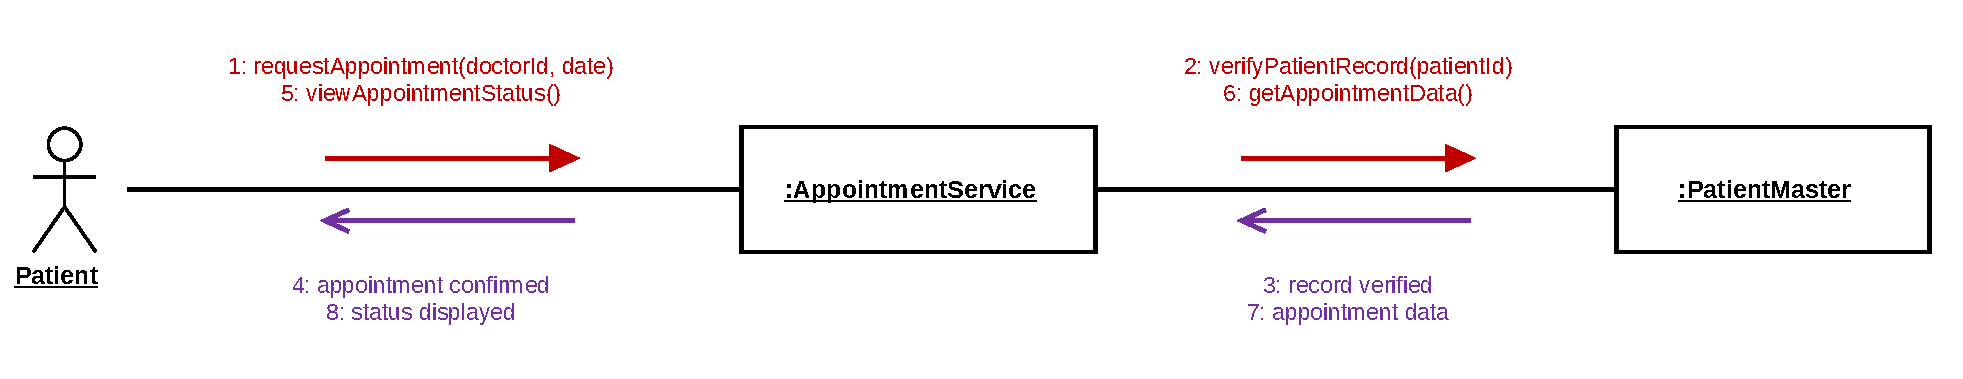
\includegraphics[width=\linewidth,height=0.82\textheight,keepaspectratio]{figures/collab1.pdf}
  \caption{Collaboration diagram 1: book appointment}
  \label{fig:collab1}
\end{figure}
\end{landscape}
\clearpage

\begin{landscape}
\section{Collaboration Diagram 2: Generate Synthetic Dataset}

\begin{figure}[H]
  \centering
  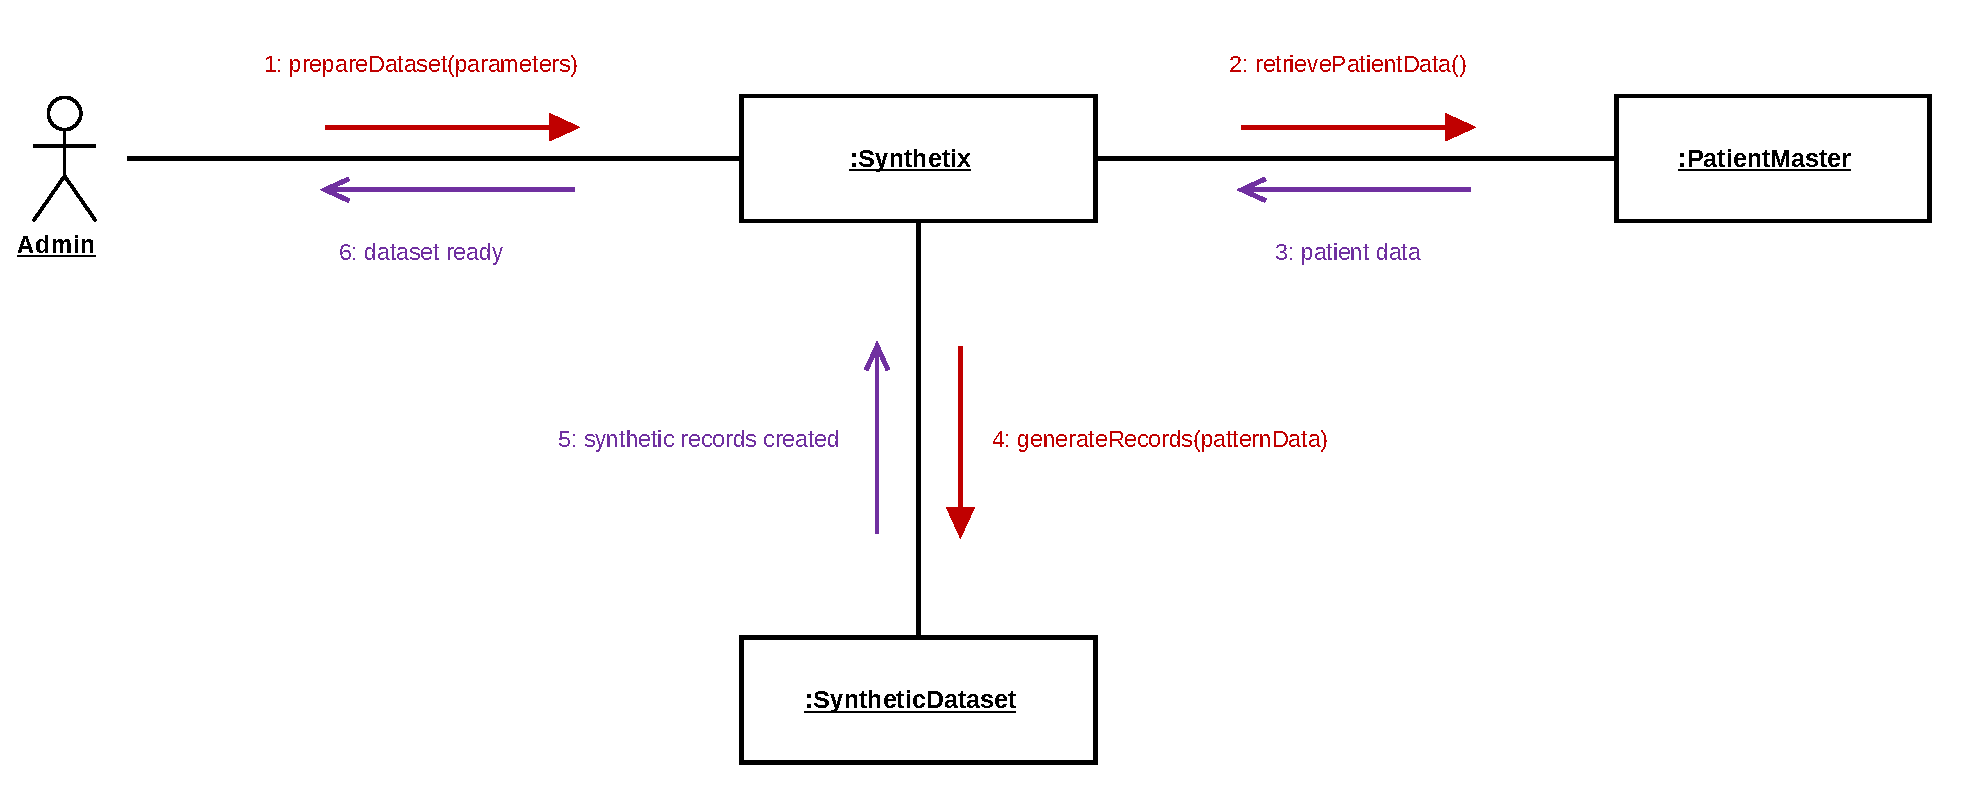
\includegraphics[width=\linewidth,height=0.82\textheight,keepaspectratio]{figures/collab2.pdf}
  \caption{Collaboration diagram 2: generate synthetic dataset}
  \label{fig:collab2}
\end{figure}
\end{landscape}
\clearpage

% ----- State diagrams -----
\begin{landscape}
\section{State Diagram 1: Appointment}

\begin{figure}[H]
  \centering
  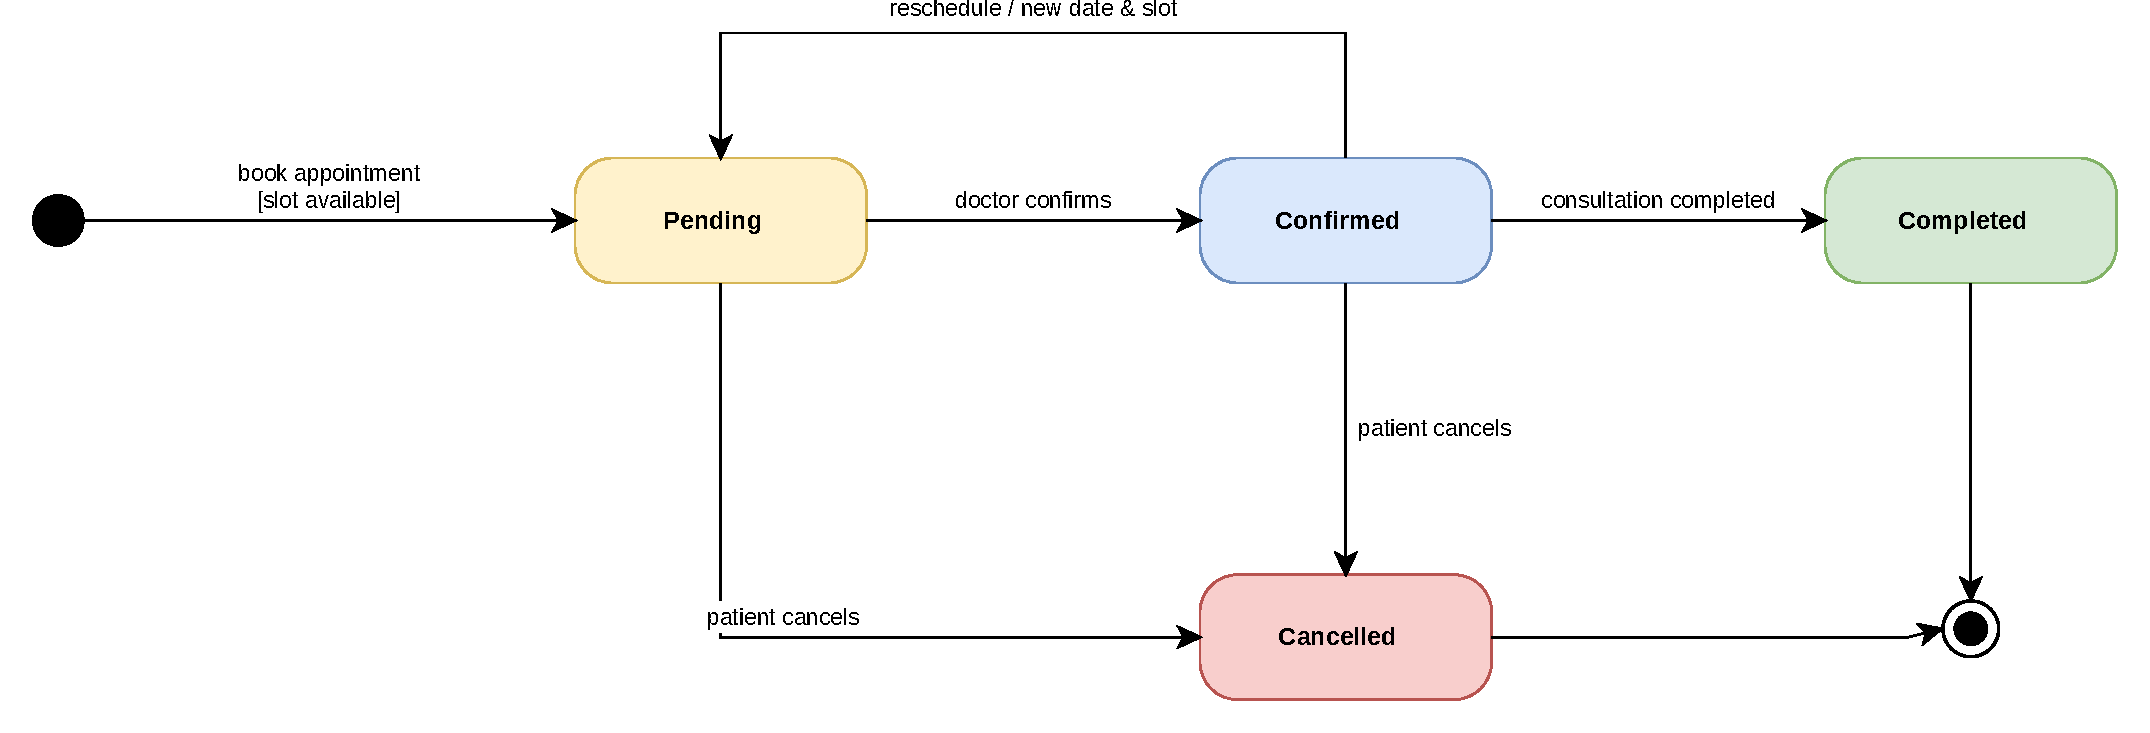
\includegraphics[width=\linewidth,height=0.82\textheight,keepaspectratio]{figures/state1.pdf}
  \caption{State diagram 1: appointment}
  \label{fig:state1}
\end{figure}
\end{landscape}
\clearpage

\begin{landscape}
\section{State Diagram 2: Bill and Payment}

\begin{figure}[H]
  \centering
  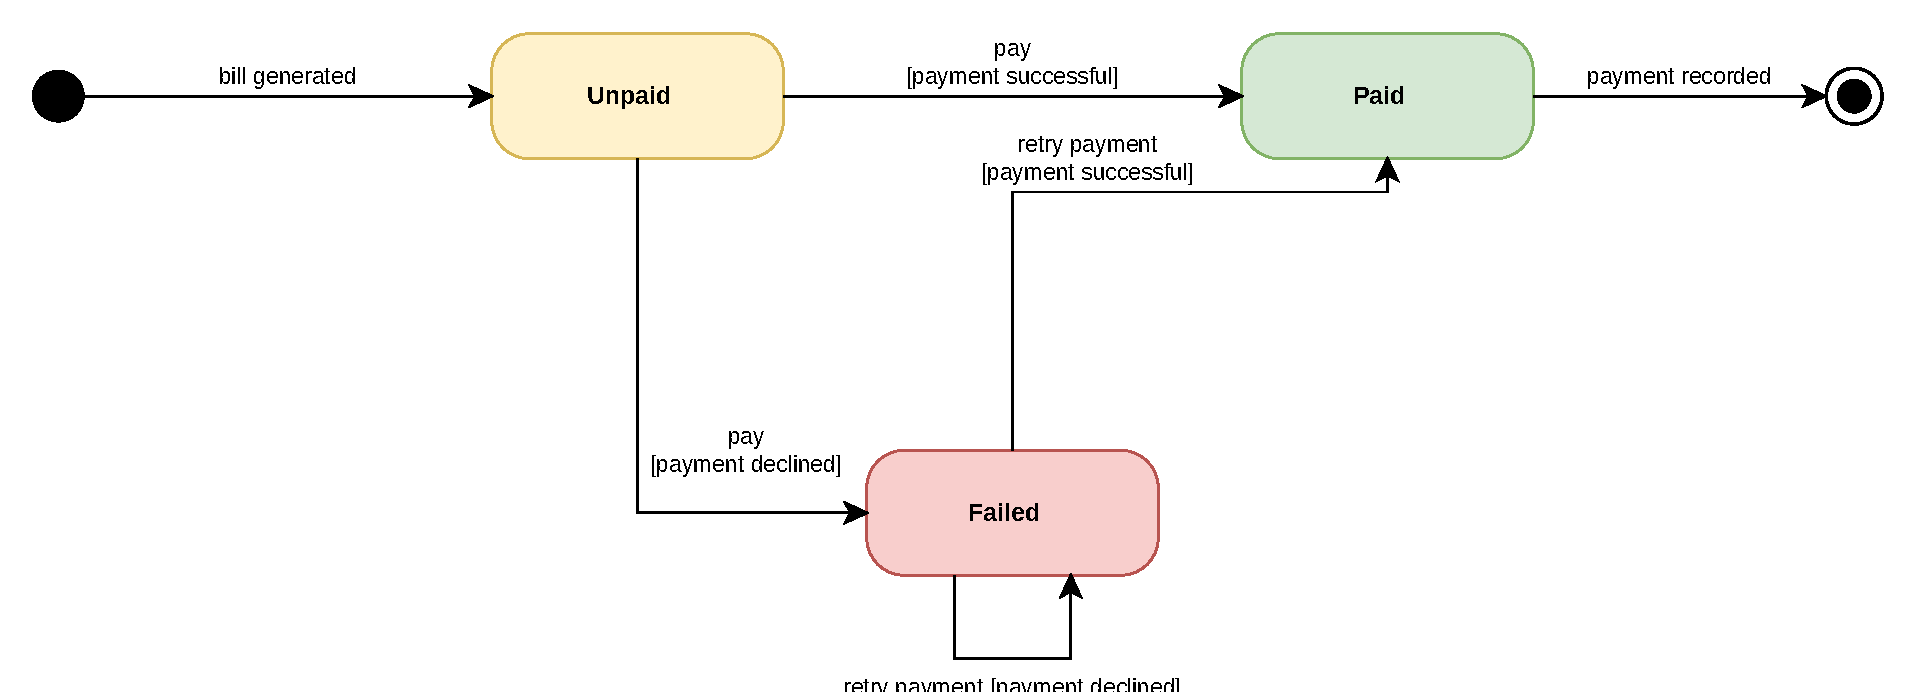
\includegraphics[width=\linewidth,height=0.82\textheight,keepaspectratio]{figures/state2.pdf}
  \caption{State diagram 2: bill and payment}
  \label{fig:state2}
\end{figure}
\end{landscape}
\clearpage

\begin{landscape}
\section{State Diagram 3: Synthetic Dataset}

\begin{figure}[H]
  \centering
  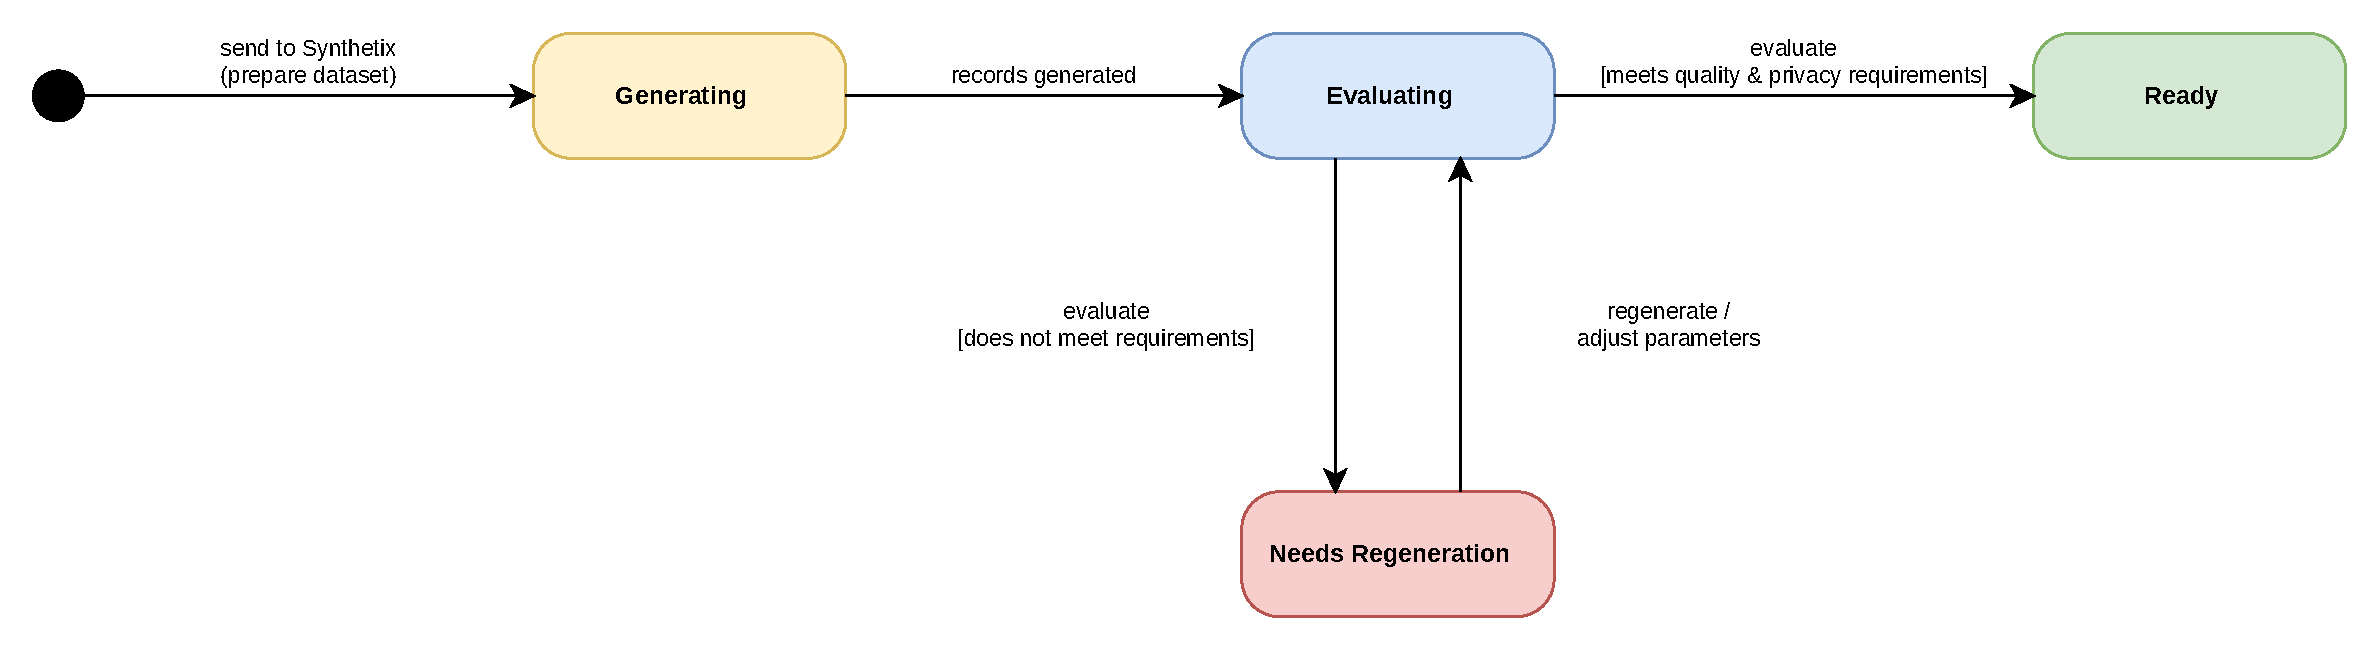
\includegraphics[width=\linewidth,height=0.82\textheight,keepaspectratio]{figures/state3.pdf}
  \caption{State diagram 3: synthetic dataset}
  \label{fig:state3}
\end{figure}
\end{landscape}
\clearpage

% ----- Component diagram -----
\begin{landscape}
\section{Component Diagram}
\begin{figure}[H]
  \centering
  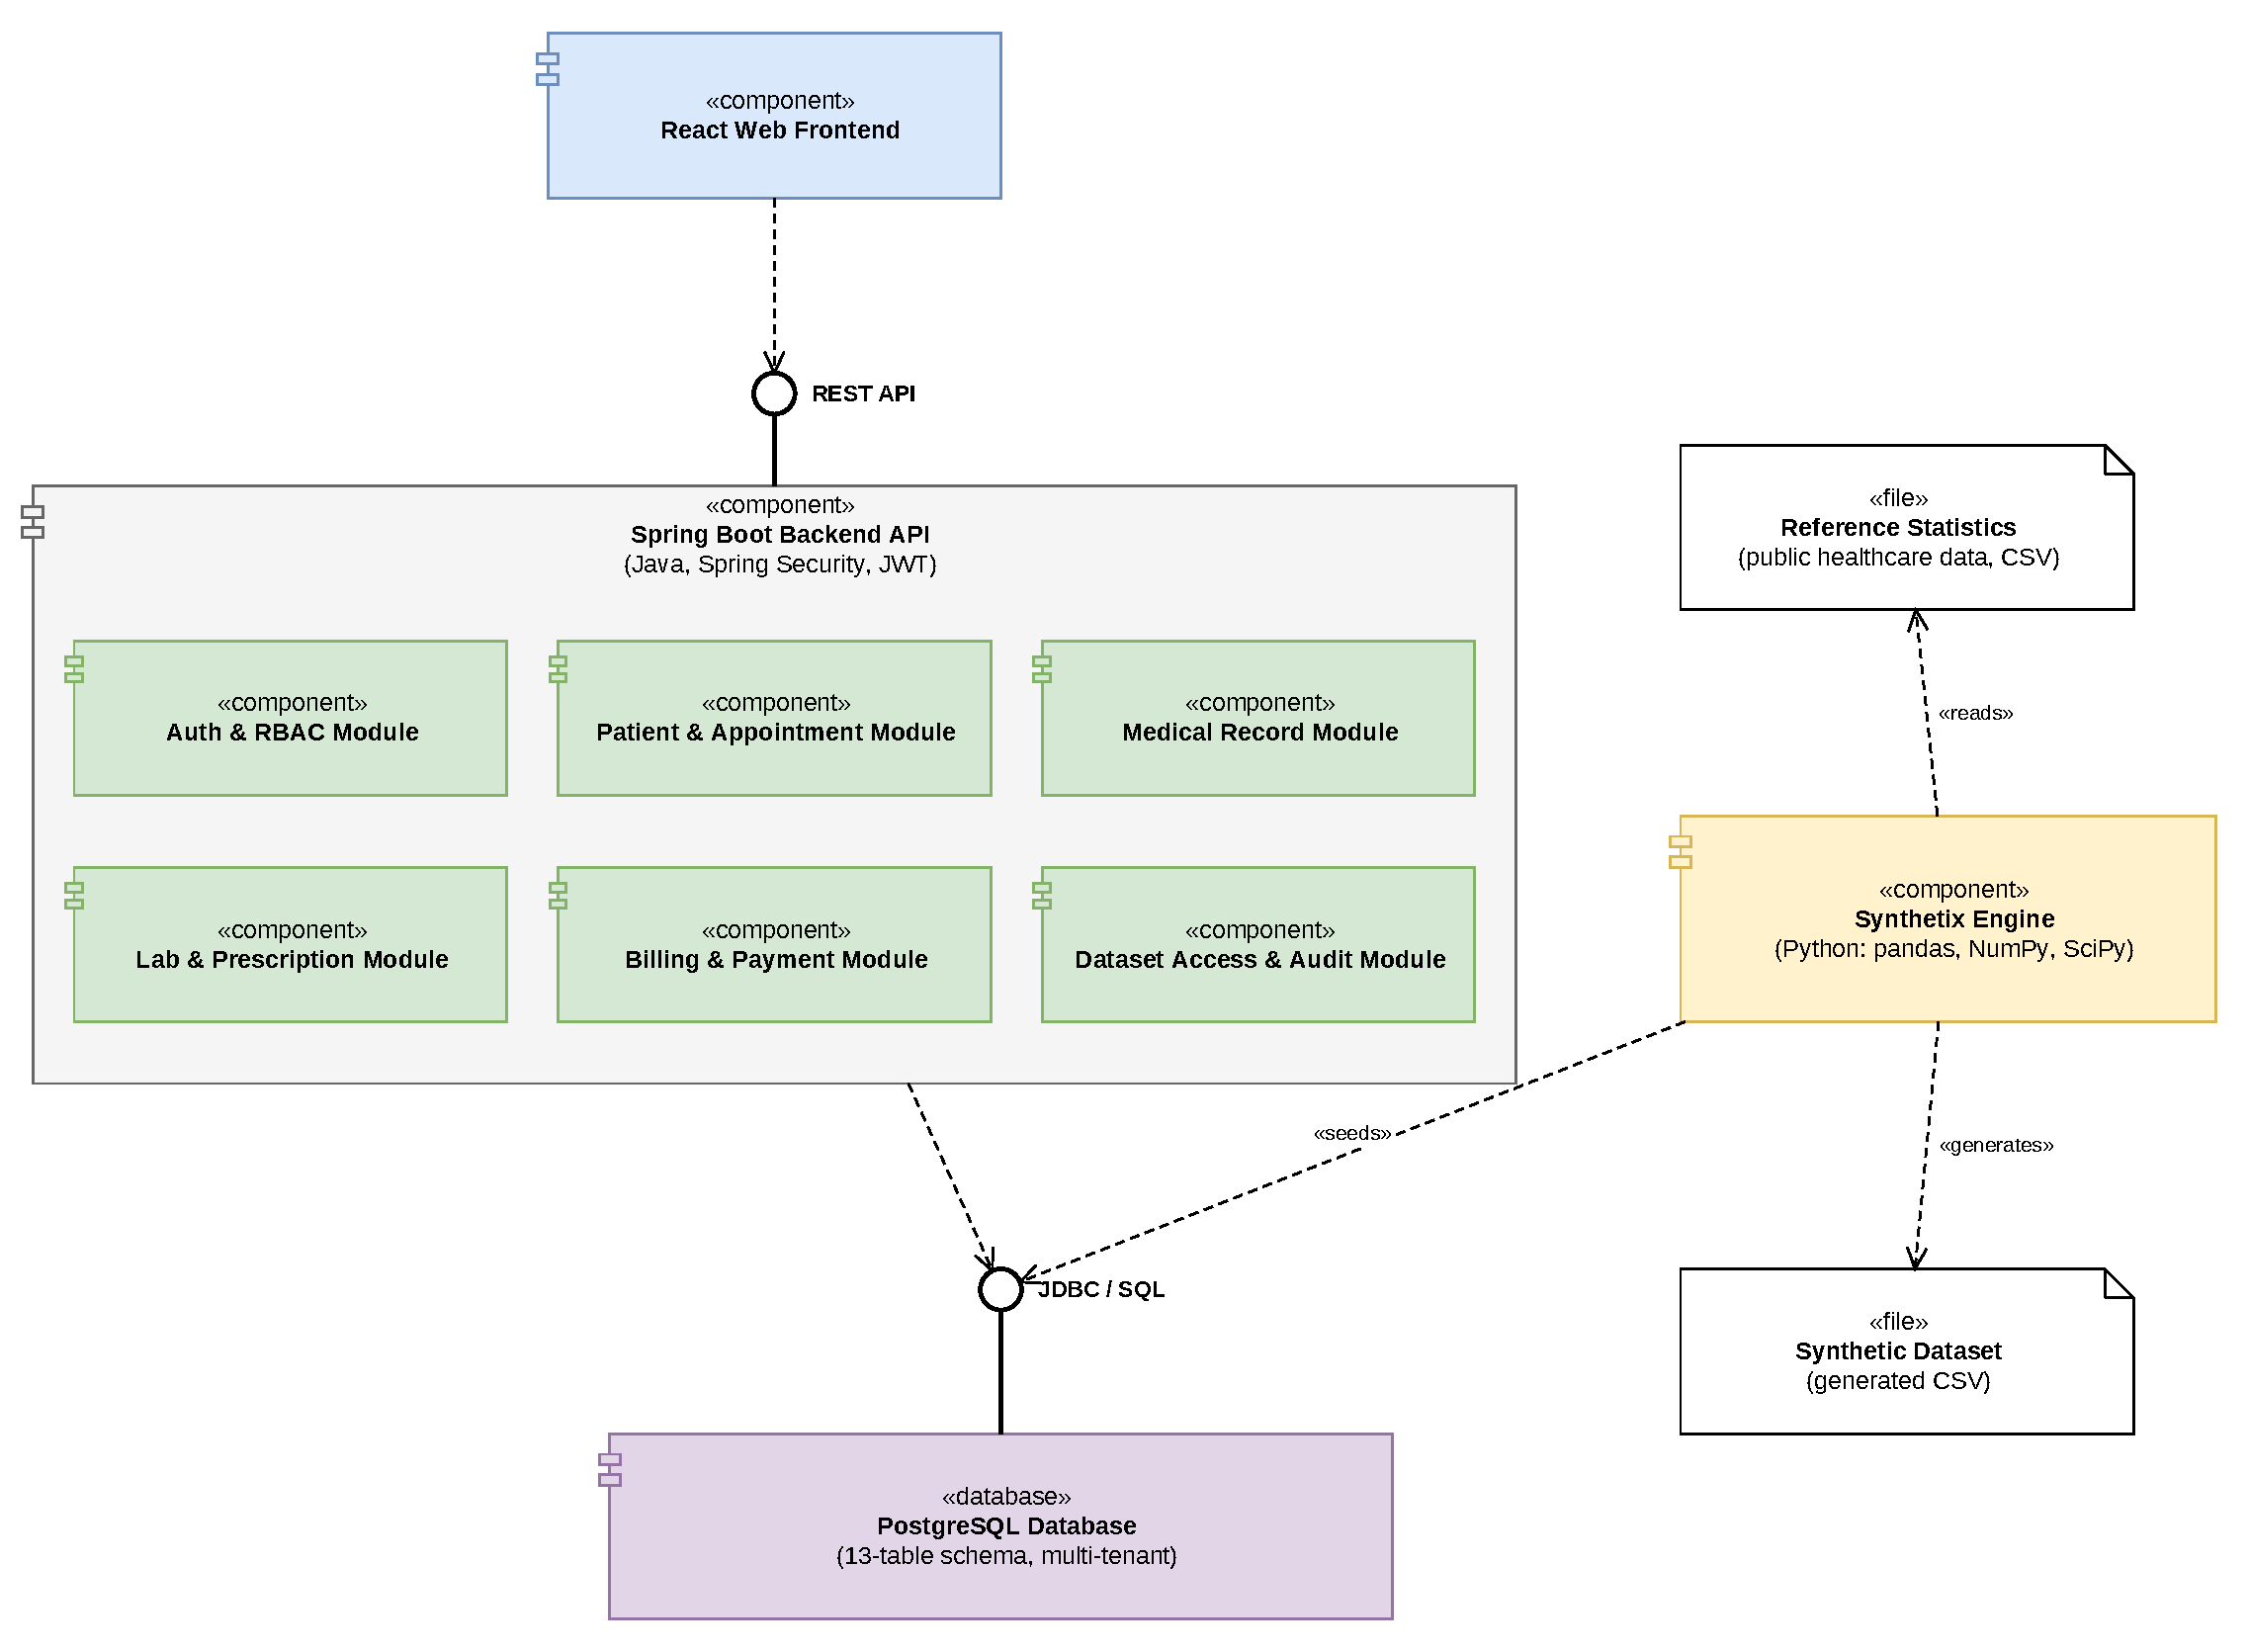
\includegraphics[width=\linewidth,height=0.82\textheight,keepaspectratio]{figures/component.pdf}
  \caption{Component diagram for MediSynth}
  \label{fig:component}
\end{figure}
\end{landscape}

% ===== BIBLIOGRAPHY =====
% Add \printbibliography[heading=bibintoc] here once biblatex is enabled above.

\end{document}
